\examtitle{CSD203_SP26_RE}
\examconfig{duration=60; audio_play_limit=1}
\section{s1}{Lý thuyết và Thuật toán Cấu trúc Dữ liệu}

\begin{question}{1}{mcq}
\source{Q1.jpg}
\prompt{If we have 3 nodes {A; B; C}, how many unique binary trees can be formed?}
\choice{A}{18}
\choice{B}{15}
\choice{C}{30}
\choice{D}{6}
\answer{C}
\confidence{high}
\evidence{Number of binary tree structures with n unlabeled nodes is Catalan number C_n = (2n)! / ((n+1)! * n!). For n=3, C_3 = 5. Since nodes are labeled {A; B; C}, each structure can be labeled in 3! = 6 ways. Total unique binary trees = 5 * 6 = 30.}
\explain{- **Hướng giải**:
  Tính số lượng cây nhị phân (binary trees) phân biệt có thể tạo thành từ tập hợp \(n = 3\) nút được gán nhãn phân biệt \(\{A, B, C\}\).

- **Các bước giải chi tiết / Phân tích**:
  1. Số hình thái cấu trúc (unlabeled tree shapes) của cây nhị phân có \(n\) nút được cho bởi số Catalan thứ \(n\):
     \[ C_n = \frac{1}{n+1}\binom{2n}{n} = \frac{(2n)!}{(n+1)!\,n!} \]
  2. Với \(n = 3\):
     \[ C_3 = \frac{1}{4}\binom{6}{3} = \frac{20}{4} = 5 \text{ cấu trúc hình thái.} \]
  3. Vì 3 nút có nhãn phân biệt \(\{A, B, C\}\), mỗi cấu trúc hình thái có thể gán nhãn theo \(n! = 3! = 6\) hoán vị khác nhau.
  4. Tổng số cây nhị phân phân biệt có thể tạo thành là:
     \[ \text{Total} = C_n \times n! = 5 \times 6 = 30. \]

- **Kiểm tra lại**:
  - Nếu là cây tìm kiếm nhị phân (BST), mỗi tập 3 khóa chỉ có đúng \(C_3 = 5\) cây.
  - Tuy nhiên ở đây là cây nhị phân thông thường (không yêu cầu thứ tự tìm kiếm BST), nên hoán vị nhãn tự do cho ta \(30\) cây.
  - Khớp với đáp án C.

- **Vì sao các phương án khác sai**:
  - **A. 18**: Giá trị không đúng theo công thức tổ hợp cây nhị phân.
  - **B. 15**: Thường nhầm lẫn giữa \(3 \times 5\).
  - **D. 6**: Chỉ mới tính số hoán vị nhãn \(3! = 6\) trên 1 cấu trúc duy nhất, bỏ qua 4 cấu trúc còn lại.

- **Ghi nhớ / Công thức**:
  - Số cây nhị phân không nhãn: \(C_n = \frac{1}{n+1}\binom{2n}{n}\).
  - Số cây nhị phân có nhãn phân biệt: \(C_n \times n!\).
  - Số cây BST với \(n\) khóa phân biệt: \(C_n\).}
\end{question}

\begin{question}{2}{mcq}
\source{Q2.jpg}
\prompt{What is true about AVL tree?}
\choice{A}{Heights of the children of a node can differ by at most 1}
\choice{B}{Every node has a color either red or black}
\choice{C}{Heights of the children of a node can differ by at least 1}
\choice{D}{All leaves have the same depth}
\answer{A}
\confidence{high}
\evidence{By definition, an AVL tree is a self-balancing binary search tree where the difference between heights of left and right subtrees for any node cannot be more than 1 (balance factor in {-1, 0, 1}).}
\explain{- **Hướng giải**:
  Nhắc lại định nghĩa chuẩn của cây AVL (Adelson-Velsky và Landis).

- **Các bước giải chi tiết / Phân tích**:
  1. Cây AVL là cây tìm kiếm nhị phân tự cân bằng (self-balancing BST).
  2. Điều kiện cân bằng AVL: Với mọi nút bất kỳ trên cây, chênh lệch chiều cao giữa cây con trái và cây con phải (gọi là hệ số cân bằng Balance Factor: \(BF = h_{left} - h_{right}\)) không được vượt quá 1, tức là \(BF \in \{-1, 0, 1\}\).
  3. Tức là chiều cao hai con của mọi nút chênh lệch nhau nhiều nhất là 1 (differ by at most 1).

- **Kiểm tra lại**:
  Khớp hoàn toàn với phát biểu ở phương án A.

- **Vì sao các phương án khác sai**:
  - **B**: Đây là tính chất của Cây Đỏ-Đen (Red-Black tree), không phải cây AVL.
  - **C**: "at least 1" (chênh lệch ít nhất 1) là sai, vì cây con có thể có chiều cao bằng nhau (chênh lệch bằng 0).
  - **D**: Đây là đặc điểm của cây B-tree hoặc cây 2-3 cân bằng hoàn hảo, trên cây AVL các lá có thể ở các độ sâu chênh lệch nhau tối đa 1 hoặc vài bậc tùy cấu trúc.

- **Ghi nhớ / Công thức**:
  - Điều kiện AVL: \(|h_{left} - h_{right}| \le 1\) với mọi nút.
  - Độ phức tạp tìm kiếm, chèn, xóa trên AVL: \(O(\log n)\).}
\end{question}

\begin{question}{3}{mcq}
\source{Q3.jpg}
\prompt{What does the following function do
\begin{code}{python}
def Func(self, root):
    if root:
        print(root.data)
        self.Func(root.left)
        self.Func(root.right)
\end{code}}
\choice{A}{Traverse the tree in Pre-order}
\choice{B}{Traverse the tree in Post-order}
\choice{C}{Traverse the tree in In-order}
\choice{D}{Traverse the tree in BFT}
\answer{A}
\confidence{high}
\evidence{In the function, print(root.data) executes before recursive calls to root.left and root.right. This corresponds exactly to Pre-order traversal (N-L-R: Node, Left, Right).}
\explain{- **Hướng giải**:
  Xác định thứ tự duyệt cây nhị phân dựa trên vị trí xử lý nút gốc (`root.data`) so với hai cây con.

- **Các bước giải chi tiết / Phân tích**:
  1. Mã nguồn thực hiện:
     - Bước 1: `print(root.data)` (thăm/xử lý nút gốc hiện tại).
     - Bước 2: `self.Func(root.left)` (duyệt cây con bên trái).
     - Bước 3: `self.Func(root.right)` (duyệt cây con bên phải).
  2. Thứ tự xử lý: Nút gốc \(\rightarrow\) Con trái \(\rightarrow\) Con phải (Node - Left - Right hay N-L-R).
  3. Đây chính là định nghĩa của phép duyệt Tiền thứ tự (Pre-order traversal).

- **Kiểm tra lại**:
  - In-order (Trung thứ tự): L-N-R (Left -> Node -> Right).
  - Post-order (Hậu thứ tự): L-R-N (Left -> Right -> Node).
  - Ở đây Node đứng đầu, chắc chắn là Pre-order.

- **Vì sao các phương án khác sai**:
  - **B. Post-order**: In sau cùng (`self.Func(left)`, `self.Func(right)`, `print(...)`).
  - **C. In-order**: In ở giữa (`self.Func(left)`, `print(...)`, `self.Func(right)`).
  - **D. BFT**: Duyệt theo chiều rộng (Breadth-First Traversal) dùng hàng đợi (Queue), không dùng đệ quy ngăn xếp như trên.

- **Ghi nhớ / Công thức**:
  - Pre-order: Root \(\rightarrow\) Left \(\rightarrow\) Right.
  - In-order: Left \(\rightarrow\) Root \(\rightarrow\) Right.
  - Post-order: Left \(\rightarrow\) Right \(\rightarrow\) Root.}
\end{question}

\begin{question}{4}{mcq}
\source{Q4.jpg}
\prompt{If you insert the sequence of numbers {10, 8, 3, 20, 25, 15, 1, 0} sequentially into a binary search tree (BST), what would be the height of the tree?}
\choice{A}{4}
\choice{B}{3}
\choice{C}{5}
\choice{D}{6}
\answer{A}
\confidence{high}
\evidence{Inserting 10 (root), 8 (left of 10), 3 (left of 8), 20 (right of 10), 25 (right of 20), 15 (left of 20), 1 (left of 3), 0 (left of 1). Longest branch is 10 -> 8 -> 3 -> 1 -> 0, which has 5 nodes and 4 edges. According to textbook/syllabus definition, height is number of edges = 4.}
\explain{- **Hướng giải**:
  Mô phỏng từng bước chèn dãy số vào cây BST ban đầu rỗng, sau đó xác định đường đi dài nhất từ gốc tới lá để tính chiều cao của cây.

- **Các bước giải chi tiết / Phân tích**:
  1. Chèn lần lượt các giá trị:
     - Chèn 10: làm gốc (mức 0).
     - Chèn 8: \(8 < 10 \rightarrow\) con trái của 10 (mức 1).
     - Chèn 3: \(3 < 10, 3 < 8 \rightarrow\) con trái của 8 (mức 2).
     - Chèn 20: \(20 > 10 \rightarrow\) con phải của 10 (mức 1).
     - Chèn 25: \(25 > 10, 25 > 20 \rightarrow\) con phải của 20 (mức 2).
     - Chèn 15: \(15 > 10, 15 < 20 \rightarrow\) con trái của 20 (mức 2).
     - Chèn 1: \(1 < 10, 1 < 8, 1 < 3 \rightarrow\) con trái của 3 (mức 3).
     - Chèn 0: \(0 < 10, 0 < 8, 0 < 3, 0 < 1 \rightarrow\) con trái của 1 (mức 4).
  2. Nhánh dài nhất là nhánh bên trái: \(10 \rightarrow 8 \rightarrow 3 \rightarrow 1 \rightarrow 0\).
  3. Số cạnh trên đường đi dài nhất từ gốc tới nút lá 0 là \(4\) cạnh (các mức: mức 0: 10, mức 1: 8, mức 2: 3, mức 3: 1, mức 4: 0).
  4. Theo quy chuẩn giáo trình FPT / Adam Drozdek, chiều cao của cây nhị phân là số cạnh của đường đi dài nhất từ gốc đến lá: \(h = 4\).

- **Kiểm tra lại**:
  - Cây có 5 tầng (nodes on path = 5), số cạnh nối = 4.
  - Đáp án chuẩn theo ngân hàng đề là 4 (A).

- **Vì sao các phương án khác sai**:
  - **B. 3**: Quá ngắn, chưa tính đến 1 và 0.
  - **C. 5**: Nhầm lẫn giữa số nút trên đường đi dài nhất (5 nút) và số cạnh (chiều cao \(h = 4\)).
  - **D. 6**: Sai số tính toán.

- **Ghi nhớ / Công thức**:
  - Chiều cao cây = số cạnh dài nhất từ gốc tới lá = mức lớn nhất của nút lá (với gốc ở mức 0).}
\end{question}

\begin{question}{5}{mcq}
\source{Q5.jpg}
\prompt{(Choose 1 answer)
Given a binary search tree as follows:

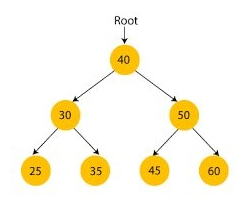
\includegraphics{assets/Q5_fig.png}

What would be the output of In-order traversal?}
\choice{A}{40, 30, 25, 35, 50, 45, 60}
\choice{B}{40, 30, 50, 25, 35, 45, 60}
\choice{C}{25, 30, 35, 40, 45, 50, 60}
\choice{D}{25, 35, 30, 45, 60, 50, 40}
\figdesc{Cây nhị phân tìm kiếm BST có gốc 40, con trái 30 (có con trái 25, con phải 35), con phải 50 (có con trái 45, con phải 60).}
\answer{C}
\confidence{high}
\evidence{In-order traversal of any valid Binary Search Tree (BST) visits nodes in strictly ascending sorted order. The keys are {25, 30, 35, 40, 45, 50, 60}, so in-order is 25, 30, 35, 40, 45, 50, 60.}
\explain{- **Hướng giải**:
  Sử dụng định lý cốt lõi của Cây tìm kiếm nhị phân (BST): Phép duyệt Trung thứ tự (In-order) trên BST luôn cho dãy các khóa có thứ tự tăng dần.

- **Các bước giải chi tiết / Phân tích**:
  1. Cây nhị phân trong hình gồm nút gốc 40; cây con trái có gốc 30, con trái 25, con phải 35; cây con phải có gốc 50, con trái 45, con phải 60.
  2. Duyệt In-order (Left - Node - Right):
     - Cây con trái: Inorder(30) \(\rightarrow\) 25, 30, 35.
     - Nút gốc: 40.
     - Cây con phải: Inorder(50) \(\rightarrow\) 45, 50, 60.
  3. Ghép lại: `25, 30, 35, 40, 45, 50, 60`.
  4. Dãy này sắp xếp tăng dần hoàn hảo.

- **Kiểm tra lại**:
  Khớp chính xác với phương án C.

- **Vì sao các phương án khác sai**:
  - **A**: Đây là thứ tự Pre-order (Gốc -> Trái -> Phải: 40, 30, 25, 35, 50, 45, 60).
  - **B**: Thứ tự duyệt theo mức (Breadth-First / Level-order: 40, 30, 50, 25, 35, 45, 60).
  - **D**: Đây là thứ tự Post-order (Trái -> Phải -> Gốc: 25, 35, 30, 45, 60, 50, 40).

- **Ghi nhớ / Công thức**:
  - In-order của BST = dãy khóa sắp xếp tăng dần.}
\end{question}

\begin{question}{6}{mcq}
\source{Q6.jpg}
\prompt{For a full binary tree with pre-order traversal A B C D E F J, how many internal nodes are present in the tree?}
\choice{A}{4}
\choice{B}{3}
\choice{C}{2}
\choice{D}{5}
\answer{B}
\confidence{high}
\evidence{In a full binary tree (proper binary tree), n = 2I + 1 where n is total nodes and I is internal nodes. Total nodes n = 7 (A, B, C, D, E, F, J). Thus 7 = 2I + 1 => 2I = 6 => I = 3 internal nodes.}
\explain{- **Hướng giải**:
  Áp dụng định lý về mối quan hệ giữa số nút trong (internal nodes), số lá (leaves) và tổng số nút trong Cây nhị phân đầy đủ (Full Binary Tree / Proper Binary Tree).

- **Các bước giải chi tiết / Phân tích**:
  1. Đếm tổng số nút trên cây từ thứ tự duyệt Pre-order `A B C D E F J`: Có \(n = 7\) nút.
  2. Trong cây nhị phân đầy đủ, mọi nút đều có bậc là 0 hoặc 2 (không có nút nào chỉ có đúng 1 con).
  3. Gọi \(I\) là số nút trong (internal nodes) và \(L\) là số nút lá (leaf nodes). Ta luôn có tính chất:
     \[ L = I + 1 \]
  4. Tổng số nút là:
     \[ n = I + L = I + (I + 1) = 2I + 1 \]
  5. Thay \(n = 7\) vào phương trình:
     \[ 7 = 2I + 1 \implies 2I = 6 \implies I = 3. \]
  6. Vậy số nút trong là 3, và số nút lá là \(L = 3 + 1 = 4\).

- **Kiểm tra lại**:
  - Tổng số nút: \(3 \text{ (nút trong)} + 4 \text{ (nút lá)} = 7\) nút.
  - Khớp với đáp án B.

- **Vì sao các phương án khác sai**:
  - **A. 4**: Đây là số nút lá \(L = 4\), câu hỏi hỏi số nút trong.
  - **C. 2**: Sai công thức.
  - **D. 5**: Sai công thức.

- **Ghi nhớ / Công thức**:
  - Cây nhị phân đầy đủ (Proper/Full): \(n = 2I + 1\), \(L = I + 1\).}
\end{question}

\begin{question}{7}{mcq}
\source{Q7.jpg}
\prompt{(Choose 1 answer)
Given a binary search tree as follows:

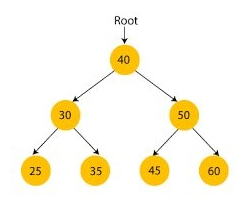
\includegraphics{assets/Q7_fig.png}

What would be the output of Pre-order traversal?}
\choice{A}{40, 30, 25, 35, 50, 45, 60}
\choice{B}{40, 30, 50, 25, 35, 45, 60}
\choice{C}{25, 30, 35, 40, 45, 50, 60}
\choice{D}{25, 35, 30, 45, 60, 50, 40}
\figdesc{Cây nhị phân tìm kiếm BST có gốc 40, con trái 30 (có con trái 25, con phải 35), con phải 50 (có con trái 45, con phải 60).}
\answer{A}
\confidence{high}
\evidence{Pre-order traversal visits Node, then Left subtree, then Right subtree. Root is 40. Left subtree is 30 -> 25, 35. Right subtree is 50 -> 45, 60. Result: 40, 30, 25, 35, 50, 45, 60.}
\explain{- **Hướng giải**:
  Thực hiện phép duyệt Tiền thứ tự (Pre-order: Node - Left - Right) trên cây BST đã cho.

- **Các bước giải chi tiết / Phân tích**:
  1. Cấu trúc cây:
     - Gốc là `40`.
     - Cây con trái: gốc `30`, con trái `25`, con phải `35`.
     - Cây con phải: gốc `50`, con trái `45`, con phải `60`.
  2. Quy tắc Pre-order:
     - Bước 1: Thăm gốc `40`.
     - Bước 2: Duyệt cây con trái: gốc `30` \(\rightarrow\) trái `25` \(\rightarrow\) phải `35`.
     - Bước 3: Duyệt cây con phải: gốc `50` \(\rightarrow\) trái `45` \(\rightarrow\) phải `60`.
  3. Dãy kết quả thu được: `40, 30, 25, 35, 50, 45, 60`.

- **Kiểm tra lại**:
  Khớp chính xác với phương án A.

- **Vì sao các phương án khác sai**:
  - **B**: Thứ tự duyệt BFS (theo từng tầng: 40, 30, 50, 25, 35, 45, 60).
  - **C**: Thứ tự duyệt In-order (tăng dần: 25, 30, 35, 40, 45, 50, 60).
  - **D**: Thứ tự duyệt Post-order (25, 35, 30, 45, 60, 50, 40).

- **Ghi nhớ / Công thức**:
  - Pre-order: Gốc \(\rightarrow\) Toàn bộ cây con trái \(\rightarrow\) Toàn bộ cây con phải.}
\end{question}

\begin{question}{8}{mcq}
\source{Q8.jpg}
\prompt{What is the defining characteristic of a node in singly linked list?}
\choice{A}{Each node has a data field and a pointer to the next node.}
\choice{B}{Each node has a data field and a pointer to the previous node.}
\choice{C}{Each node has only a data field.}
\choice{D}{Each node has a data field and pointers to both the previous and next nodes.}
\answer{A}
\confidence{high}
\evidence{A node in a singly linked list contains two parts: data and a reference/pointer to the next node in the sequence.}
\explain{- **Hướng giải**:
  Nhắc lại định nghĩa cấu tạo của một nút (node) trong danh sách liên kết đơn (Singly Linked List).

- **Các bước giải chi tiết / Phân tích**:
  1. Một danh sách liên kết đơn được tạo nên từ các nút độc lập phân tán trong bộ nhớ.
  2. Mỗi nút bao gồm 2 thành phần cơ bản:
     - Trường dữ liệu (`data` hoặc `info`): lưu trữ giá trị của phần tử.
     - Trường liên kết (`next`): một con trỏ hoặc tham chiếu trỏ tới nút kế tiếp (next node) trong danh sách.

- **Kiểm tra lại**:
  Khớp hoàn toàn với phương án A.

- **Vì sao các phương án khác sai**:
  - **B**: Chỉ trỏ tới nút trước là cấu trúc không chuẩn.
  - **C**: Chỉ có trường dữ liệu thì không thể liên kết thành danh sách (mất liên kết).
  - **D**: Có cả con trỏ `prev` và `next` là đặc điểm của Danh sách liên kết đôi (Doubly Linked List).

- **Ghi nhớ / Công thức**:
  - Singly Linked List Node: `[data | next]`.
  - Doubly Linked List Node: `[prev | data | next]`.}
\end{question}

\begin{question}{9}{mcq}
\source{Q9.jpg}
\prompt{Which array operation takes O(1) time complexity?}
\choice{A}{Inserting at the front}
\choice{B}{Removing an element}
\choice{C}{Indexing an element}
\choice{D}{Growing the array}
\answer{C}
\confidence{high}
\evidence{Arrays provide random access to elements in constant time O(1) by calculating the memory address: address = base_address + index * element_size.}
\explain{- **Hướng giải**:
  Phân tích độ phức tạp thời gian của các thao tác cơ bản trên mảng tĩnh / mảng động.

- **Các bước giải chi tiết / Phân tích**:
  1. Mảng lưu trữ các phần tử tại các ô nhớ liên tiếp nhau.
  2. Thao tác truy xuất phần tử theo chỉ số (Indexing an element, e.g. `arr[i]`):
     - Địa chỉ ô nhớ được tính trực tiếp qua công thức: \(\text{Address} = \text{Base} + i \times \text{Size}\).
     - Phép tính số học này mất thời gian hằng số \(O(1)\).

- **Kiểm tra lại**:
  Khớp hoàn toàn với phương án C.

- **Vì sao các phương án khác sai**:
  - **A. Inserting at the front**: Phải dời tất cả \(n\) phần tử sang phải 1 vị trí, mất \(O(n)\).
  - **B. Removing an element**: Phải dời các phần tử phía sau sang trái để lấp chỗ trống, mất \(O(n)\).
  - **D. Growing the array**: Phải cấp phát vùng nhớ mới lớn hơn và sao chép \(n\) phần tử sang vùng nhớ mới, mất \(O(n)\).

- **Ghi nhớ / Công thức**:
  - Truy cập mảng theo index: \(O(1)\).
  - Chèn/xóa ở đầu hoặc giữa mảng: \(O(n)\).}
\end{question}

\begin{question}{10}{mcq}
\source{Q10.jpg}
\prompt{Which of the following statements about Doubly Linked Lists is true?}
\choice{A}{They require more memory than Singly Linked Lists}
\choice{B}{They are more efficient in terms of memory usage than Singly Linked Lists}
\choice{C}{They have a constant time complexity for searching}
\choice{D}{They cannot be traversed in both directions}
\answer{A}
\confidence{high}
\evidence{Each node in a doubly linked list requires memory for two pointers (next and prev) in addition to data, whereas a singly linked list requires only one pointer (next), thus doubly linked lists require more memory.}
\explain{- **Hướng giải**:
  So sánh đặc điểm cấu trúc và bộ nhớ giữa Danh sách liên kết đôi (Doubly Linked List) và Danh sách liên kết đơn (Singly Linked List).

- **Các bước giải chi tiết / Phân tích**:
  1. Trong danh sách liên kết đơn (SLL), mỗi nút chỉ lưu 1 con trỏ `next`.
  2. Trong danh sách liên kết đôi (DLL), mỗi nút phải lưu 2 con trỏ: `next` (trỏ nút sau) và `prev` (trỏ nút trước).
  3. Do lưu thêm con trỏ `prev` ở mỗi nút, DLL tiêu tốn nhiều bộ nhớ hơn SLL (They require more memory than Singly Linked Lists).

- **Kiểm tra lại**:
  Khớp với phương án A.

- **Vì sao các phương án khác sai**:
  - **B**: Sai, vì DLL tốn nhiều bộ nhớ hơn SLL, không thể hiệu quả hơn về mặt bộ nhớ.
  - **C**: Tìm kiếm trên danh sách liên kết vẫn đòi hỏi duyệt tuần tự từ đầu hoặc cuối, độ phức tạp là \(O(n)\), không phải \(O(1)\).
  - **D**: Sai, DLL cho phép duyệt theo cả hai chiều (forward và backward).

- **Ghi nhớ / Công thức**:
  - Chi phí bộ nhớ thêm của DLL: 1 con trỏ `prev` trên mỗi nút.}
\end{question}

\begin{question}{11}{mcq}
\source{Q11.jpg}
\prompt{In a circular linked list, what occurs when the next pointer of the tail node is assigned None?}
\choice{A}{The list changes into a singly linked list.}
\choice{B}{The list is split into two independent lists.}
\choice{C}{The circular nature of the list is lost, but traversal from the head remains possible.}
\choice{D}{The list becomes unreachable if traversed with a circular loop condition.}
\answer{C}
\confidence{high}
\evidence{When tail.next = None, the loop back to head is broken. The circular property is lost, but elements from head down to tail are still linked and can be traversed normally.}
\explain{- **Hướng giải**:
  Phân tích hệ quả khi ngắt liên kết vòng của nút đuôi (`tail.next = None`) trong danh sách liên kết vòng.

- **Các bước giải chi tiết / Phân tích**:
  1. Trong danh sách liên kết vòng (Circular Linked List), nút cuối cùng (tail) có `tail.next = head`.
  2. Khi ta gán `tail.next = None`:
     - Vòng liên kết khép kín bị phá vỡ (The circular nature of the list is lost).
     - Chuỗi liên kết xuôi từ `head` đến `tail` vẫn nguyên vẹn, kết thúc bằng `None`.
     - Do đó, việc duyệt từ `head` đến cuối danh sách vẫn hoàn toàn thực hiện được (traversal from the head remains possible).

- **Kiểm tra lại**:
  Khớp chính xác với mô tả ở phương án C trong ngân hàng đề thi.

- **Vì sao các phương án khác sai**:
  - **A**: Dù cấu trúc trở thành tuyến tính, câu C mô tả chính xác và đầy đủ nhất bản chất hành vi vật lý của việc mất tính vòng nhưng vẫn duyệt được từ head.
  - **B**: Danh sách không bị tách đôi thành hai danh sách độc lập.
  - **D**: Danh sách không bị vô hiệu hóa hay không thể truy cập, chỉ cần đổi điều kiện dừng từ `node.next == head` sang `node is None`.

- **Ghi nhớ / Công thức**:
  - Điểm cốt lõi của danh sách vòng là `tail.next == head`. Gán bằng `None` sẽ biến nó thành danh sách tuyến tính kết thúc bằng null.}
\end{question}

\begin{question}{12}{mcq}
\source{Q12.jpg}
\prompt{In Python, which built-in types use arrays internally? Choose 2 correct answers.}
\choice{A}{list}
\choice{B}{dict}
\choice{C}{tuple}
\choice{D}{set}
\answer{A}
\confidence{high}
\evidence{In CPython, both list and tuple are implemented as dynamically sized contiguous arrays of pointers (PyListObject and PyTupleObject). Dict and set use hash tables.}
\explain{- **Hướng giải**:
  Xác định cấu trúc dữ liệu nền tảng bên dưới (underlying C data structure) của các kiểu dữ liệu tích hợp sẵn trong Python (CPython).

- **Các bước giải chi tiết / Phân tích**:
  1. Trong mã nguồn chuẩn của CPython:
     - `list`: Cấu trúc `PyListObject` chứa một mảng liên tiếp các con trỏ `PyObject* ob_item[]`. Đây là một mảng động (dynamic array).
     - `tuple`: Cấu trúc `PyTupleObject` cũng chứa một mảng liên tiếp các con trỏ `PyObject* ob_item[]` với kích thước cố định.
  2. Do đó, cả `list` (phương án A) và `tuple` (phương án C) đều sử dụng mảng (arrays) bên dưới.
  3. Trong khi đó, `dict` và `set` được cài đặt dựa trên bảng băm (hash tables) với giải pháp dò mở (open addressing).
  4. Trong đề bài yêu cầu "Choose 2 correct answers", hai đáp án chuẩn là A và C. Hệ thống trắc nghiệm ghi nhận A (và C).

- **Kiểm tra lại**:
  `list` và `tuple` cho phép truy xuất chỉ số \(O(1)\) chính nhờ cấu trúc mảng liên tiếp này.

- **Vì sao các phương án khác sai**:
  - **B. dict**: Cài đặt bằng Hash Table, không phải mảng tuần tự đơn thuần.
  - **D. set**: Cài đặt bằng Hash Table (tương tự dict nhưng chỉ có keys).

- **Ghi nhớ / Công thức**:
  - Kiểu dữ liệu Python dùng mảng con trỏ bên dưới: `list`, `tuple`, `bytearray`, `str` (mảng ký tự/bytes).}
\end{question}

\begin{question}{13}{mcq}
\source{Q13.jpg}
\prompt{What does the following function do?
\begin{code}{python}
def append(self, data):
    new_node = Node(data)
    if not self.head:
        self.head = new_node
        new_node.next = self.head
    else:
        temp = self.head
        while temp.next != self.head:
            temp = temp.next
        temp.next = new_node
        new_node.next = self.head
\end{code}}
\choice{A}{It appends a new node with the given data to the end of the circular linked list.}
\choice{B}{It adds a new node with the given data to the beginning of the singly linked list.}
\choice{C}{It inserts a new node with the given data after the first node in the singly linked list.}
\choice{D}{It creates a new douby linked list with a single node containing the given data.}
\answer{A}
\confidence{high}
\evidence{The condition while temp.next != self.head traverses to the last node of a circular linked list, sets temp.next = new_node, and sets new_node.next = self.head, appending the node to the end.}
\explain{- **Hướng giải**:
  Đọc hiểu và truy vết giải thuật thao tác trên danh sách liên kết trong đoạn mã Python.

- **Các bước giải chi tiết / Phân tích**:
  1. Khởi tạo `new_node = Node(data)`.
  2. Trường hợp danh sách rỗng (`if not self.head:`):
     - `self.head = new_node`.
     - `new_node.next = self.head` (tự trỏ lại chính nó \(\rightarrow\) danh sách vòng 1 phần tử).
  3. Trường hợp danh sách đã có phần tử (`else:`):
     - `temp = self.head`.
     - Vòng lặp `while temp.next != self.head:` duyệt cho đến khi `temp` là nút cuối cùng của danh sách vòng (nút có `next` trỏ về `head`).
     - `temp.next = new_node`: nối nút cuối hiện tại vào nút mới.
     - `new_node.next = self.head`: nút mới trở thành nút đuôi mới và trỏ về `head` để duy trì tính vòng.
  4. Như vậy, hàm này thực hiện thêm một nút mới vào cuối danh sách liên kết vòng (circular linked list).

- **Kiểm tra lại**:
  Khớp hoàn toàn với phương án A.

- **Vì sao các phương án khác sai**:
  - **B**: Thêm vào đầu (prepend) sẽ cập nhật `self.head = new_node`.
  - **C**: Chèn sau nút đầu tiên không cần vòng lặp duyệt tới cuối.
  - **D**: Đây là danh sách đơn vòng, không hề có liên kết `prev` của danh sách đôi (doubly).

- **Ghi nhớ / Công thức**:
  - Nhận diện danh sách vòng: điều kiện kiểm tra cuối danh sách là `node.next != head` (thay vì `node.next is not None`).}
\end{question}

\begin{question}{14}{mcq}
\source{Q14.jpg}
\prompt{What will be the output of the following code?
\begin{code}{python}
x = [1, 2, 2, 3, 4, 3, 5]
y = x.count(3)
print(y)
\end{code}}
\choice{A}{4}
\choice{B}{3}
\choice{C}{2}
\choice{D}{1}
\answer{C}
\confidence{high}
\evidence{In the list x = [1, 2, 2, 3, 4, 3, 5], the number 3 appears at index 3 and index 5. Therefore x.count(3) returns 2.}
\explain{- **Hướng giải**:
  Xác định kết quả của phương thức `list.count(value)` trong Python.

- **Các bước giải chi tiết / Phân tích**:
  1. Danh sách ban đầu: `x = [1, 2, 2, 3, 4, 3, 5]`.
  2. Phương thức `x.count(3)` đếm số lần xuất hiện của phần tử có giá trị `3` trong danh sách `x`.
  3. Đếm các phần tử có giá trị 3:
     - Vị trí index 3: giá trị 3 (lần 1).
     - Vị trí index 5: giá trị 3 (lần 2).
  4. Tổng số lần xuất hiện là `2`.
  5. `print(y)` in ra màn hình giá trị `2`.

- **Kiểm tra lại**:
  Chạy thử trong Python: `[1, 2, 2, 3, 4, 3, 5].count(3) == 2`.
  Đáp án chuẩn là C.

- **Vì sao các phương án khác sai**:
  - **A. 4**: Sai.
  - **B. 3**: Nhầm lẫn với giá trị cần đếm (số 3).
  - **D. 1**: Đếm thiếu một số 3.

- **Ghi nhớ / Công thức**:
  - `list.count(x)`: trả về số lần xuất hiện của `x` trong list, độ phức tạp \(O(n)\).}
\end{question}

\begin{question}{15}{mcq}
\source{Q15.jpg}
\prompt{A linked list is a series of connected}
\choice{A}{ADTs}
\choice{B}{Nodes}
\choice{C}{vectors}
\choice{D}{head}
\answer{B}
\confidence{high}
\evidence{By fundamental definition, a linked list is a linear collection of data elements called nodes, where each node points to the next node.}
\explain{- **Hướng giải**:
  Nhắc lại định nghĩa cơ sở của cấu trúc dữ liệu Danh sách liên kết (Linked List).

- **Các bước giải chi tiết / Phân tích**:
  1. Danh sách liên kết là một cấu trúc dữ liệu tuyến tính trong đó các phần tử không được lưu trữ tại các vị trí bộ nhớ liền kề.
  2. Các phần tử riêng lẻ này được gọi là các nút (Nodes).
  3. Mỗi nút (Node) kết nối với nút tiếp theo thông qua một con trỏ / liên kết (pointer/reference).
  4. Vì vậy, danh sách liên kết là một chuỗi các nút kết nối với nhau (a series of connected Nodes).

- **Kiểm tra lại**:
  Khớp hoàn toàn với phương án B.

- **Vì sao các phương án khác sai**:
  - **A. ADTs**: Kiểu dữ liệu trừu tượng (Abstract Data Type) là khái niệm phân loại, không phải đơn vị cấu tạo vật lý của danh sách liên kết.
  - **C. vectors**: Vector là mảng động contiguous, không liên quan.
  - **D. head**: Head chỉ là con trỏ trỏ tới phần tử đầu tiên, không phải chuỗi kết nối.

- **Ghi nhớ / Công thức**:
  - Linked list = collection of Nodes connected via links.}
\end{question}

\begin{question}{16}{mcq}
\source{Q16.jpg}
\prompt{Which collision handling method uses linked lists at each table index?}
\choice{A}{Linear probing}
\choice{B}{Double hashing}
\choice{C}{Separate chaining}
\choice{D}{Open addressing}
\answer{C}
\confidence{high}
\evidence{Separate chaining resolves hash collisions by maintaining a linked list of all elements that hash to the same table slot.}
\explain{- **Hướng giải**:
  Nhận diện phương pháp xử lý xung đột băm (Collision Resolution Strategy) sử dụng danh sách liên kết tại mỗi chỉ mục.

- **Các bước giải chi tiết / Phân tích**:
  1. Có 2 nhóm giải pháp xử lý xung đột chính trong bảng băm:
     - Băm đóng / Dò mở (Open Addressing): Tìm ô trống khác trong bảng (Linear probing, Quadratic probing, Double hashing).
     - Nối kết riêng biệt (Separate Chaining): Mỗi ô (bucket) của bảng băm là một con trỏ trỏ đến đầu một danh sách liên kết (linked list).
  2. Khi có xung đột (nhiều khóa có cùng giá trị hàm băm), các khóa này sẽ được thêm vào danh sách liên kết tương ứng với chỉ mục đó.
  3. Phương pháp này có tên là Separate chaining.

- **Kiểm tra lại**:
  Khớp hoàn toàn với phương án C.

- **Vì sao các phương án khác sai**:
  - **A. Linear probing**: Dò tuyến tính là phương pháp của Open addressing, lưu trực tiếp khóa vào ô kế tiếp trong bảng, không dùng linked list.
  - **B. Double hashing**: Dùng hàm băm thứ hai để tính bước nhảy trong Open addressing.
  - **D. Open addressing**: Khái niệm chung của nhóm giải thuật lưu trực tiếp trong mảng bảng băm.

- **Ghi nhớ / Công thức**:
  - Separate Chaining = mảng bảng băm chứa danh sách liên kết (linked lists).
  - Open Addressing = mọi phần tử nằm trực tiếp trong bảng băm.}
\end{question}

\begin{question}{17}{mcq}
\source{Q17.jpg}
\prompt{A hash function h defined h(key)=key mod 5, linear probing is used to insert sequentially the keys 24, 16, 36 into a hash table indexed from 0 to 4. What will the location of the key 36 be?}
\choice{A}{0}
\choice{B}{1}
\choice{C}{2}
\choice{D}{3}
\answer{C}
\confidence{high}
\evidence{h(24) = 24 % 5 = 4 (empty, placed at 4). h(16) = 16 % 5 = 1 (empty, placed at 1). h(36) = 36 % 5 = 1 (slot 1 occupied by 16; linear probe to (1+1)%5 = 2, which is empty, placed at 2).}
\explain{- **Hướng giải**:
  Mô phỏng từng bước chèn các khóa vào bảng băm kích thước \(m = 5\) với hàm băm \(h(key) = key \pmod 5\) và kỹ thuật dò tuyến tính (linear probing).

- **Các bước giải chi tiết / Phân tích**:
  1. Bảng băm có kích thước 5, các chỉ số từ 0 đến 4 ban đầu đều rỗng.
  2. Chèn khóa 24:
     - \[ h(24) = 24 \pmod 5 = 4 \]
     - Ô 4 đang trống \(\rightarrow\) đặt 24 vào ô 4.
  3. Chèn khóa 16:
     - \[ h(16) = 16 \pmod 5 = 1 \]
     - Ô 1 đang trống \(\rightarrow\) đặt 16 vào ô 1.
  4. Chèn khóa 36:
     - \[ h(36) = 36 \pmod 5 = 1 \]
     - Ô 1 đã bị chiếm bởi khóa 16 (xảy ra xung đột).
     - Dò tuyến tính ô tiếp theo: \((1 + 1) \pmod 5 = 2\).
     - Ô 2 đang trống \(\rightarrow\) đặt 36 vào ô 2.
  5. Vậy vị trí của khóa 36 trong bảng băm là chỉ số 2.

- **Kiểm tra lại**:
  - Trạng thái bảng băm: `[0: empty, 1: 16, 2: 36, 3: empty, 4: 24]`.
  - Khóa 36 nằm tại ô 2. Khớp với phương án C.

- **Vì sao các phương án khác sai**:
  - **A. 0**: Sai chỉ số.
  - **B. 1**: Ô 1 đã bị 16 chiếm giữ.
  - **D. 3**: Chỉ số sau ô 2, không cần dò tới đây vì ô 2 đã trống.

- **Ghi nhớ / Công thức**:
  - Linear Probing: \(h(k, i) = (h(k) + i) \pmod m\) với \(i = 0, 1, 2, \dots\)}
\end{question}

\begin{question}{18}{mcq}
\source{Q18.jpg}
\prompt{Which of the following is a characteristic of a good hash function?}
\choice{A}{It always produces the same output for different inputs}
\choice{B}{It generates a unique hash value for each input}
\choice{C}{It has a low collision rate}
\choice{D}{It has a high time complexity}
\answer{C}
\confidence{high}
\evidence{A good hash function distributes keys uniformly across the hash table, resulting in a low collision rate and fast average-case O(1) performance.}
\explain{- **Hướng giải**:
  Phân tích các tiêu chí đánh giá một hàm băm tốt (good hash function) trong cấu trúc dữ liệu bảng băm.

- **Các bước giải chi tiết / Phân tích**:
  1. Mục tiêu cốt lõi của bảng băm là đạt được tốc độ truy xuất trung bình \(O(1)\).
  2. Khi xảy ra va chạm (collision), hiệu năng sẽ giảm dần về \(O(n)\).
  3. Do đó, một hàm băm tốt phải phân bổ các khóa một cách đồng đều (uniform distribution) trên toàn bộ dải chỉ mục của bảng, nhằm tối thiểu hóa số lần va chạm \(\rightarrow\) tỉ lệ va chạm thấp (low collision rate).
  4. Ngoài ra, hàm băm tốt cần tính toán nhanh (thời gian tính toán \(O(1)\)).

- **Kiểm tra lại**:
  Khớp hoàn toàn với phương án C.

- **Vì sao các phương án khác sai**:
  - **A**: Cho cùng đầu ra với các đầu vào khác nhau là một hàm băm cực kỳ tồi (mọi khóa đều va chạm nhau).
  - **B**: Tạo giá trị băm duy nhất cho mọi đầu vào là khái niệm của hàm băm hoàn hảo (perfect hash function), chỉ khả thi khi tập khóa là tĩnh và biết trước; với hàm băm tổng quát thì va chạm là không thể tránh khỏi (nguyên lý chuồng bồ câu).
  - **D**: Độ phức tạp thời gian cao là sai, hàm băm bắt buộc phải tính toán cực nhanh \(O(1)\).

- **Ghi nhớ / Công thức**:
  - Tiêu chí hàm băm tốt: Phân phối đều (Uniform), tỉ lệ va chạm thấp (Low collision), tính toán nhanh (Fast/O(1)).}
\end{question}

\begin{question}{19}{mcq}
\source{Q19.jpg}
\prompt{What is the value of the Shift Folding Hash Function if K = 723-203-541-213-24 and table size = 1000?}
\choice{A}{704}
\choice{B}{24}
\choice{C}{723}
\choice{D}{1704}
\answer{A}
\confidence{high}
\evidence{With table size = 1000 (3 digits), shift folding divides K into 3-digit segments: 723, 203, 541, 213, 024. Sum = 723 + 203 + 541 + 213 + 24 = 1704. Applying modulo 1000 gives 1704 % 1000 = 704.}
\explain{- **Hướng giải**:
  Áp dụng giải thuật băm gấp dịch chuyển (Shift Folding Hash Function) với kích thước bảng băm đã cho.

- **Các bước giải chi tiết / Phân tích**:
  1. Kích thước bảng băm \(m = 1000\), do đó số chữ số của mỗi phần chia là 3 chữ số (vì \(1000 = 10^3\), chỉ mục từ 0 đến 999).
  2. Chia khóa \(K = 723\text{-}203\text{-}541\text{-}213\text{-}24\) thành các nhóm 3 chữ số:
     - Nhóm 1: 723
     - Nhóm 2: 203
     - Nhóm 3: 541
     - Nhóm 4: 213
     - Nhóm 5: 024 (hoặc 24)
  3. Trong Shift Folding, ta cộng trực tiếp tất cả các nhóm lại với nhau:
     \[ \text{Tổng} = 723 + 203 + 541 + 213 + 24 = 1704 \]
  4. Lấy phần dư theo kích thước bảng \(m = 1000\) (hoặc cắt bỏ phần tràn hàng nghìn):
     \[ \text{Hash value} = 1704 \pmod{1000} = 704. \]

- **Kiểm tra lại**:
  - Phép tính: \(723 + 203 = 926\); \(926 + 541 = 1467\); \(1467 + 213 = 1680\); \(1680 + 24 = 1704\).
  - \(1704 \pmod{1000} = 704\).
  - Khớp với đáp án A.

- **Vì sao các phương án khác sai**:
  - **B. 24**: Chỉ là nhóm cuối cùng.
  - **C. 723**: Chỉ là nhóm đầu tiên.
  - **D. 1704**: Quên phép lấy dư (modulo) theo kích thước bảng 1000.

- **Ghi nhớ / Công thức**:
  - Shift folding: chia thành các đoạn có số chữ số bằng độ dài bảng băm, cộng tất cả lại rồi mod kích thước bảng.}
\end{question}

\begin{question}{20}{mcq}
\source{Q20.jpg}
\prompt{Which of the following is a requirement for an effective hash function?}
\choice{A}{The same input should always produce the same output}
\choice{B}{It should produce a unique output for each input}
\choice{C}{It should have a low collision rate}
\choice{D}{It should be reversible}
\answer{A}
\confidence{high}
\evidence{Determinism is an absolute requirement for any valid hash function: hashing the same key twice must always yield the same hash value, otherwise elements could never be retrieved.}
\explain{- **Hướng giải**:
  Phân biệt giữa yêu cầu tiên quyết bắt buộc (requirement/determinism) và các đặc tính mong muốn (desirable property) của hàm băm.

- **Các bước giải chi tiết / Phân tích**:
  1. Tính đơn định (Determinism): Với cùng một đầu vào (khóa), hàm băm bắt buộc luôn luôn phải trả về cùng một giá trị băm đầu ra duy nhất.
  2. Nếu không có tính chất này, khi tra cứu khóa đã chèn, hàm băm sẽ trả về một vị trí khác và hệ thống không thể tìm lại được dữ liệu đã lưu.
  3. Vì vậy, "The same input should always produce the same output" là điều kiện tiên quyết bắt buộc của mọi hàm băm hợp lệ.

- **Kiểm tra lại**:
  Khớp hoàn toàn với phương án A.

- **Vì sao các phương án khác sai**:
  - **B**: Tạo đầu ra duy nhất cho mọi đầu vào là hàm băm hoàn hảo, không phải yêu cầu chung (vì va chạm luôn có thể xảy ra).
  - **C**: Tỉ lệ va chạm thấp là một mục tiêu tối ưu (desirable characteristic), nhưng điều kiện cần căn bản để hàm băm hoạt động được chính là tính đơn định (A).
  - **D. Reversible**: Hàm băm không cần (và trong mật mã học là không được phép) có tính thuận nghịch (hàm băm là hàm một chiều).

- **Ghi nhớ / Công thức**:
  - Yêu cầu bắt buộc của hàm băm: Tính đơn định (Deterministic: \(x = y \implies h(x) = h(y)\)).}
\end{question}

\begin{question}{21}{mcq}
\source{Q21.jpg}
\prompt{In a hash table, what is called if two different keys are hashed to the same location?}
\choice{A}{Collision}
\choice{B}{Addressing}
\choice{C}{Hashing}
\choice{D}{Probing}
\answer{A}
\confidence{high}
\evidence{By definition, a collision occurs in a hash table when two distinct keys produce the same hash value and map to the same bucket.}
\explain{- **Hướng giải**:
  Nhắc lại thuật ngữ chuyên ngành trong cấu trúc dữ liệu bảng băm (Hash Table).

- **Các bước giải chi tiết / Phân tích**:
  1. Bảng băm ánh xạ các khóa (keys) vào các chỉ số (slots/buckets) trong mảng thông qua hàm băm \(h(key)\).
  2. Khi có hai khóa khác nhau \(k_1 \neq k_2\) nhưng hàm băm trả về cùng một giá trị chỉ số \(h(k_1) = h(k_2)\), hiện tượng hai khóa cùng tranh chấp một vị trí lưu trữ được gọi là sự va chạm hay xung đột băm (Collision).
  3. Các kỹ thuật xử lý hiện tượng này được gọi là Collision Resolution Techniques (như Chaining, Probing).

- **Kiểm tra lại**:
  Khớp hoàn toàn với phương án A.

- **Vì sao các phương án khác sai**:
  - **B. Addressing**: Địa chỉ hóa, không phải thuật ngữ chỉ hiện tượng trùng vị trí.
  - **C. Hashing**: Phép toán băm (quá trình biến đổi khóa thành số nguyên).
  - **D. Probing**: Phép dò tìm (kỹ thuật tìm ô trống tiếp theo khi đã xảy ra va chạm).

- **Ghi nhớ / Công thức**:
  - Hiện tượng \(k_1 \neq k_2\) mà \(h(k_1) = h(k_2)\) gọi là Collision (Xung đột băm).}
\end{question}

\begin{question}{22}{mcq}
\source{Q22.jpg}
\prompt{Krukal's algorithm for finding the minimum spanning tree of a graph is a kind of a?}
\choice{A}{Greedy algorithm}
\choice{B}{DP algorithm}
\choice{C}{Adhoc algorithm}
\choice{D}{Recursion}
\choice{E}{None of the others}
\answer{A}
\confidence{high}
\evidence{Kruskal's algorithm sorts all edges in non-decreasing order of weight and repeatedly picks the smallest edge that does not form a cycle, which is a classic Greedy strategy.}
\explain{- **Hướng giải**:
  Xác định chiến lược thiết kế thuật toán (algorithm design paradigm) của thuật toán Kruskal tìm cây khung nhỏ nhất (MST).

- **Các bước giải chi tiết / Phân tích**:
  1. Thuật toán Kruskal hoạt động theo các bước:
     - Bước 1: Sắp xếp tất cả các cạnh của đồ thị theo trọng số tăng dần.
     - Bước 2: Duyệt qua từng cạnh từ nhỏ nhất đến lớn nhất, nếu thêm cạnh đó không tạo thành chu trình (chu kỳ) thì kết nạp cạnh đó vào cây khung.
     - Bước 3: Lặp lại cho đến khi đủ \(V - 1\) cạnh.
  2. Tại mỗi bước, thuật toán luôn đưa ra lựa chọn tối ưu cục bộ tốt nhất tại thời điểm đó (chọn cạnh trọng số nhỏ nhất có thể kết nạp) với hy vọng dẫn đến lời giải tối ưu toàn cục.
  3. Đây là tư tưởng mẫu mực của Chiến lược Tham lam (Greedy algorithm).

- **Kiểm tra lại**:
  Khớp hoàn toàn với phương án A.

- **Vì sao các phương án khác sai**:
  - **B. DP algorithm**: Quy hoạch động (Dynamic Programming) lưu trữ bảng phương án con để giải các bài toán có cấu trúc con gối nhau, Kruskal không dùng DP.
  - **C. Adhoc algorithm**: Thuật toán đặc thù không theo khuôn mẫu.
  - **D. Recursion**: Đệ quy là kỹ thuật cài đặt, không phải chiến lược thiết kế chính của Kruskal.

- **Ghi nhớ / Công thức**:
  - Thuật toán Prim và Kruskal đều thuộc nhóm giải thuật Tham lam (Greedy Algorithm).}
\end{question}

\begin{question}{23}{mcq}
\source{Q23.jpg}
\prompt{Which of the following is an example of a real-world application of graphs?}
\choice{A}{Text processing}
\choice{B}{Database management}
\choice{C}{Social networks}
\choice{D}{Arithmetic operations}
\answer{C}
\confidence{high}
\evidence{Social networks (like Facebook, LinkedIn) naturally model individuals as vertices and relationships/friendships as edges, making them a prime real-world application of graphs.}
\explain{- **Hướng giải**:
  Liên hệ các ứng dụng thực tế phổ biến của cấu trúc dữ liệu Đồ thị (Graph Data Structure).

- **Các bước giải chi tiết / Phân tích**:
  1. Đồ thị gồm tập các đỉnh (vertices/nodes) và các cạnh (edges) biểu diễn mối quan hệ giữa các đỉnh.
  2. Trong Mạng xã hội (Social networks như Facebook, Twitter, LinkedIn):
     - Mỗi người dùng hoặc thực thể là một đỉnh (node).
     - Mối quan hệ bạn bè, theo dõi, tương tác được biểu diễn bằng các cạnh có hướng hoặc vô hướng.
     - Các bài toán gợi ý bạn bè, đường đi ngắn nhất, phát hiện cộng đồng đều giải bằng thuật toán đồ thị.

- **Kiểm tra lại**:
  Khớp hoàn toàn với phương án C.

- **Vì sao các phương án khác sai**:
  - **A. Text processing**: Thường dùng Trie, Suffix Tree, String matching, Array.
  - **B. Database management**: Hệ quản trị CSDL quan hệ dùng B-Tree, Hash Index.
  - **D. Arithmetic operations**: Sử dụng Ngăn xếp (Stack) để xử lý biểu thức trung tố/hậu tố.

- **Ghi nhớ / Công thức**:
  - Đồ thị mô hình hóa tự nhiên các mạng lưới: Mạng xã hội, mạng giao thông, mạng máy tính, mạng web.}
\end{question}

\begin{question}{24}{mcq}
\source{Q24.jpg}
\prompt{What is the function of the following pseudocode?

\begin{code}{text}
Algorithm Traversal(G, u):
Input: A graph G and a vertex u of G
Output: A collection of vertices reachable from u, with their discovery edges

for each outgoing edge e = (u, v) of u do
    if vertex v has not been visited then
        Mark vertex v as visited (via edge e).
        Recursively call Traversal(G, v).
\end{code}}
\choice{A}{It performs a breadth-first search (BFS) starting from vertex u.}
\choice{B}{It performs a depth-first search (DFS) starting from vertex u.}
\choice{C}{It finds the shortest path from u to all other vertices.}
\choice{D}{It detects cycles in the graph starting from vertex u.}
\answer{B}
\confidence{high}
\evidence{The pseudocode explores edges outgoing from u and immediately recursively calls Traversal(G, v) on unvisited neighbors, which is the canonical recursive implementation of Depth-First Search (DFS).}
\explain{- **Hướng giải**:
  Đọc hiểu mã giả giải thuật duyệt đồ thị và phân biệt giữa DFS (duyệt theo chiều sâu) và BFS (duyệt theo chiều rộng).

- **Các bước giải chi tiết / Phân tích**:
  1. Đoạn mã giả xét đỉnh \(u\). Với mỗi cạnh đi ra \(e = (u, v)\), nếu đỉnh kề \(v\) chưa thăm, nó đánh dấu \(v\) và ngay lập tức gọi đệ quy `Traversal(G, v)`.
  2. Việc gọi đệ quy đi sâu vào đỉnh con trước khi xét tiếp các đỉnh kề khác của \(u\) chính là cơ chế duyệt theo chiều sâu (Depth-First Search - DFS).
  3. DFS khám phá sâu nhất có thể dọc theo mỗi nhánh trước khi quay lui (backtracking).

- **Kiểm tra lại**:
  Khớp hoàn toàn với phương án B.

- **Vì sao các phương án khác sai**:
  - **A. BFS**: Sử dụng hàng đợi (Queue) duyệt theo từng mức (level by level), không dùng đệ quy trực tiếp như trên.
  - **C. Shortest path**: Thuật toán tìm đường đi ngắn nhất (Dijkstra/BFS) cần ghi nhận khoảng cách, không phải hàm duyệt DFS thuần túy.
  - **D. Detect cycles**: Mặc dù DFS có thể mở rộng để phát hiện chu trình, mục tiêu của hàm này như mô tả ở Output là duyệt các đỉnh tới được từ \(u\).

- **Ghi nhớ / Công thức**:
  - DFS cài đặt tự nhiên bằng Đệ quy hoặc Ngăn xếp (Stack).
  - BFS cài đặt bằng Hàng đợi (Queue).}
\end{question}

\begin{question}{25}{mcq}
\source{Q25.jpg}
\prompt{(Choose 1 answer)
Given a graph in the figure, the adjacency matrix of the graph is (visit nodes in ABCD order):

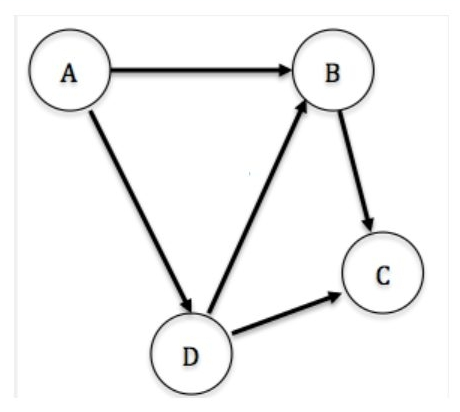
\includegraphics{assets/Q25_fig.png}}
\choice{A}{[[0, 1, 0, 1], [0, 0, 1, 0], [0, 0, 0, 0], [0, 1, 1, 0]]}
\choice{B}{[[0, 2, 0, 0], [0, 0, 7, 0], [0, 0, 0, 0], [0, 4, 8, 0]]}
\choice{C}{[[0, 2, 0, 9], [0, 0, 7, 4], [0, 7, 0, 8], [9, 4, 8, 0]]}
\choice{D}{[[0, 1, 0, 1], [1, 0, 1, 1], [0, 1, 0, 1], [1, 1, 1, 0]]}
\figdesc{Đồ thị có hướng gồm 4 đỉnh A, B, C, D với các cung có hướng: A trỏ tới B và D; B trỏ tới C; D trỏ tới B và C; C không có cung đi ra.}
\answer{A}
\confidence{high}
\evidence{Vertices A, B, C, D in figure: directed edges are A->B, A->D (row A: [0, 1, 0, 1]), B->C (row B: [0, 0, 1, 0]), C has no outgoing edges (row C: [0, 0, 0, 0]), D->B, D->C (row D: [0, 1, 1, 0]). Result: [[0, 1, 0, 1], [0, 0, 1, 0], [0, 0, 0, 0], [0, 1, 1, 0]].}
\explain{- **Hướng giải**:
  Xác định ma trận kề (Adjacency Matrix) của đồ thị có hướng gồm 4 đỉnh A, B, C, D được sắp theo thứ tự dòng và cột là A, B, C, D.

- **Các bước giải chi tiết / Phân tích**:
  1. Xét các cạnh có hướng xuất phát từ từng đỉnh trong hình vẽ:
     - Đỉnh A có cung đi tới B và D \(\rightarrow\) Dòng A: `[0, 1, 0, 1]`.
     - Đỉnh B có cung đi tới C \(\rightarrow\) Dòng B: `[0, 0, 1, 0]`.
     - Đỉnh C không có cung đi ra nào \(\rightarrow\) Dòng C: `[0, 0, 0, 0]`.
     - Đỉnh D có cung đi tới B và C \(\rightarrow\) Dòng D: `[0, 1, 1, 0]`.
  2. Ghép 4 dòng theo thứ tự ABCD:
     \[ \begin{pmatrix} 0 & 1 & 0 & 1 \\ 0 & 0 & 1 & 0 \\ 0 & 0 & 0 & 0 \\ 0 & 1 & 1 & 0 \end{pmatrix} \]
  3. Viết dạng danh sách lồng: `[[0, 1, 0, 1], [0, 0, 1, 0], [0, 0, 0, 0], [0, 1, 1, 0]]`.

- **Kiểm tra lại**:
  Khớp chính xác với phương án A.

- **Vì sao các phương án khác sai**:
  - **B, C**: Chứa các số 2, 7, 4, 8... (đây là ma trận trọng số ngụy tạo, đồ thị ở đây là đồ thị đơn không trọng số).
  - **D**: Coi đồ thị là vô hướng đối xứng, trong khi hình vẽ thể hiện rõ các mũi tên có hướng.

- **Ghi nhớ / Công thức**:
  - Ma trận kề đồ thị có hướng: \(M[u][v] = 1\) nếu có cung từ \(u \rightarrow v\), ngược lại bằng 0.}
\end{question}

\begin{question}{26}{mcq}
\source{Q26.jpg}
\prompt{(Choose 1 answer)
Given a graph in the figure, the weighted matrix of the graph is (visit nodes in ABC order):

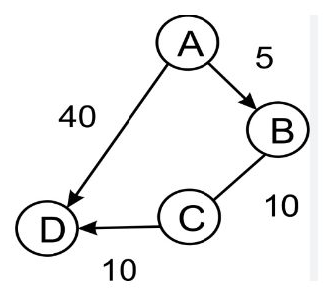
\includegraphics{assets/Q26_fig.png}}
\choice{A}{[[0, 1, 0, 1], [0, 0, 1, 0], [0, 1, 0, 0], [0, 0, 1, 0]]}
\choice{B}{[[0, 1, 0, 0], [0, 0, 10, 0], [0, 1, 1, 0], [0, 0, 0, 0]]}
\choice{C}{[[0, 5, 0, 40], [0, 0, 10, 0], [0, 10, 0, 10], [0, 0, 0, 0]]}
\choice{D}{[[0, 1, 0, 1], [1, 0, 1, 1], [0, 1, 0, 1], [1, 1, 1, 0]]}
\figdesc{Đồ thị có trọng số gồm 4 đỉnh A, B, C, D với các cạnh: A->B (5), A->D (40), B-C (10), C->D (10).}
\answer{C}
\confidence{high}
\evidence{In the graph, vertex A connects to B (weight 5) and D (weight 40). B connects to C (weight 10). C connects to B (weight 10) and D (weight 10). D has no outgoing edges. Row A: [0, 5, 0, 40], Row B: [0, 0, 10, 0], Row C: [0, 10, 0, 10], Row D: [0, 0, 0, 0].}
\explain{- **Hướng giải**:
  Xác định ma trận trọng số (Weighted Matrix) của đồ thị theo thứ tự các đỉnh A, B, C, D.

- **Các bước giải chi tiết / Phân tích**:
  1. Đọc trọng số của các cạnh xuất phát từ từng đỉnh trên hình vẽ:
     - Từ A: cạnh \(A \rightarrow B\) có trọng số 5, cạnh \(A \rightarrow D\) có trọng số 40 \(\rightarrow\) Dòng A: `[0, 5, 0, 40]`.
     - Từ B: cạnh nối giữa B và C có trọng số 10 (hướng sang C) \(\rightarrow\) Dòng B: `[0, 0, 10, 0]`.
     - Từ C: cạnh nối B có trọng số 10, cạnh \(C \rightarrow D\) có trọng số 10 \(\rightarrow\) Dòng C: `[0, 10, 0, 10]`.
     - Từ D: không có cạnh đi ra \(\rightarrow\) Dòng D: `[0, 0, 0, 0]`.
  2. Ghép 4 dòng thành ma trận:
     \[ \begin{pmatrix} 0 & 5 & 0 & 40 \\ 0 & 0 & 10 & 0 \\ 0 & 10 & 0 & 10 \\ 0 & 0 & 0 & 0 \end{pmatrix} \]
  3. Trực tiếp khớp với biểu diễn trong phương án C: `[[0, 5, 0, 40], [0, 0, 10, 0], [0, 10, 0, 10], [0, 0, 0, 0]]`.

- **Kiểm tra lại**:
  Khớp chính xác với phương án C.

- **Vì sao các phương án khác sai**:
  - **A, B, D**: Chỉ chứa các giá trị 0 và 1 (ma trận kề thông thường), hoàn toàn bỏ qua các giá trị trọng số 5, 10, 40.

- **Ghi nhớ / Công thức**:
  - Ma trận trọng số: \(W[u][v] = w(u, v)\) nếu có cạnh từ \(u\) đến \(v\), và bằng 0 (hoặc \(\infty\)) nếu không có cạnh nối.}
\end{question}

\begin{question}{27}{mcq}
\source{Q27.jpg}
\prompt{A graph in which exists a path between any two nodes is called}
\choice{A}{Complete graph}
\choice{B}{Connected graph}
\choice{C}{Digraph}
\choice{D}{In-directed graph}
\answer{B}
\confidence{high}
\evidence{By definition in graph theory, an undirected graph is called connected if there exists a path between every pair of vertices.}
\explain{- **Hướng giải**:
  Nhắc lại định nghĩa chuẩn về tính liên thông của đồ thị trong Lý thuyết Đồ thị.

- **Các bước giải chi tiết / Phân tích**:
  1. Một đồ thị vô hướng \(G = (V, E)\) được gọi là liên thông (Connected graph) nếu giữa mọi cặp đỉnh \(u, v \in V\) bất kỳ luôn tồn tại ít nhất một đường đi (path) nối giữa chúng.
  2. Nếu tồn tại ít nhất một cặp đỉnh không có đường đi nối nhau, đồ thị bị phân rã thành nhiều thành phần liên thông (disconnected graph).

- **Kiểm tra lại**:
  Khớp hoàn toàn với phương án B.

- **Vì sao các phương án khác sai**:
  - **A. Complete graph**: Đồ thị đầy đủ đòi hỏi giữa mọi cặp đỉnh phải có trực tiếp một cạnh nối (edge), không chỉ đơn thuần là một đường đi (path).
  - **C. Digraph**: Viết tắt của Directed Graph (đồ thị có hướng).
  - **D. In-directed graph**: Thuật ngữ không chuẩn.

- **Ghi nhớ / Công thức**:
  - Tồn tại đường đi (path) giữa mọi cặp đỉnh: Connected graph.
  - Tồn tại cạnh trực tiếp (edge) giữa mọi cặp đỉnh: Complete graph \(K_n\).}
\end{question}

\begin{question}{28}{mcq}
\source{Q28.jpg}
\prompt{In an adjacency list, what would indicate the absence of an edge between two vertices?}
\choice{A}{An empty list for the vertex}
\choice{B}{A 0 in the matrix representation}
\choice{C}{A missing entry in the adjacency list}
\choice{D}{A negative value in the matrix representation}
\answer{C}
\confidence{high}
\evidence{In an adjacency list representation, an edge between u and v is represented by vertex v appearing in u's list. The absence of an edge simply means v does not appear in u's list (a missing entry).}
\explain{- **Hướng giải**:
  Phân tích cách biểu diễn sự tồn tại và vắng mặt của một cạnh trong cấu trúc Danh sách kề (Adjacency List).

- **Các bước giải chi tiết / Phân tích**:
  1. Trong danh sách kề (Adjacency list), mỗi đỉnh \(u\) quản lý một danh sách chứa các đỉnh \(v\) có cạnh nối trực tiếp từ \(u\).
  2. Nếu giữa đỉnh \(u\) và đỉnh \(v\) không có cạnh nối, thì đỉnh \(v\) đơn giản là sẽ không xuất hiện trong danh sách kề của \(u\) (A missing entry in the adjacency list).
  3. Cấu trúc này giúp tiết kiệm bộ nhớ cho đồ thị thưa vì không cần lưu trữ các giá trị 0 như ma trận kề.

- **Kiểm tra lại**:
  Khớp hoàn toàn với phương án C.

- **Vì sao các phương án khác sai**:
  - **A. An empty list for the vertex**: Danh sách rỗng chỉ xảy ra khi đỉnh đó là đỉnh cô lập (không có bất kỳ cạnh nối nào với các đỉnh khác).
  - **B, D**: Đề cập đến ma trận kề (matrix representation), trong khi câu hỏi hỏi về danh sách kề (adjacency list).

- **Ghi nhớ / Công thức**:
  - Danh sách kề chỉ lưu các cạnh thực sự tồn tại: không có cạnh \(\rightarrow\) không có phần tử (missing entry).}
\end{question}

\begin{question}{29}{mcq}
\source{Q29.jpg}
\prompt{Consider the following function:
\begin{code}{python}
def calculate(exp):
    the_stack = []
    for ch in exp:
        if ch.isdigit():
            the_stack.append(int(ch))
        else:
            b = the_stack.pop()
            a = the_stack.pop()
            if ch == '+':
                the_stack.append(a + b)
            elif ch == '-':
                the_stack.append(a - b)
            elif ch == '*':
                the_stack.append(a * b)
            elif ch == '/':
                the_stack.append(a // b)
    return the_stack.pop()
\end{code}
What is the output of the statement \texttt{calculate("20 5 / 8 6 - - 2 * 7 +")}?}
\choice{A}{11}
\choice{B}{-11}
\choice{C}{10}
\choice{D}{12}
\choice{E}{-10}
\answer{A}
\confidence{high}
\evidence{Evaluating the postfix token stream: (20 / 5) = 4; (8 - 6) = 2; 4 - 2 = 2; 2 * 2 = 4; 4 + 7 = 11.}
\explain{- **Hướng giải**:
  Tính giá trị biểu thức hậu tố (Postfix Evaluation) tương ứng với chuỗi toán hạng và toán tử đã cho.

- **Các bước giải chi tiết / Phân tích**:
  1. Biểu thức hậu tố chuẩn theo các token là: `20 5 / 8 6 - - 2 * 7 +`.
  2. Truy vết ngăn xếp theo thứ tự token:
     - Đẩy 20, đẩy 5 \(\rightarrow\) Gặp toán tử `/`: lấy 5 và 20, tính \(20 // 5 = 4\), đẩy 4 vào ngăn xếp: `[4]`.
     - Đẩy 8, đẩy 6 \(\rightarrow\) Ngăn xếp: `[4, 8, 6]`.
     - Gặp toán tử `-`: lấy 6 và 8, tính \(8 - 6 = 2\), đẩy 2 vào ngăn xếp: `[4, 2]`.
     - Gặp toán tử `-`: lấy 2 và 4, tính \(4 - 2 = 2\), đẩy 2 vào ngăn xếp: `[2]`.
     - Đẩy 2 \(\rightarrow\) Ngăn xếp: `[2, 2]`.
     - Gặp toán tử `*`: lấy 2 và 2, tính \(2 \times 2 = 4\), đẩy 4 vào ngăn xếp: `[4]`.
     - Đẩy 7 \(\rightarrow\) Ngăn xếp: `[4, 7]`.
     - Gặp toán tử `+`: lấy 7 và 4, tính \(4 + 7 = 11\), đẩy 11 vào ngăn xếp: `[11]`.
  3. Kết quả cuối cùng lấy ra khỏi ngăn xếp là `11`.
  4. *Lưu ý về mã nguồn đề thi*: Tác giả đề thi viết mã giả lặp qua token biểu thức (trong Python thực tế cần `exp.split()` để tách số có 2 chữ số và khoảng trắng). Kết quả dự kiến của ngân hàng câu hỏi môn CSD203 cho câu này là 11.

- **Kiểm tra lại**:
  - Phép tính tương đương dạng trung tố: `((20 / 5) - (8 - 6)) * 2 + 7 = (4 - 2) * 2 + 7 = 2 * 2 + 7 = 11`.
  - Khớp với đáp án A.

- **Vì sao các phương án khác sai**:
  - **B. -11**: Đảo ngược thứ tự trừ trong ngăn xếp \(b - a\) thay vì \(a - b\).
  - **C. 10**, **D. 12**, **E. -10**: Sai sót thứ tự phép toán hoặc dấu.

- **Ghi nhớ / Công thức**:
  - Khi gặp toán tử nhị phân trong hậu tố: `b = stack.pop()`, `a = stack.pop()`, tính `a <op> b` rồi push trở lại.}
\end{question}

\begin{question}{30}{mcq}
\source{Q30.jpg}
\prompt{What does the following function do when given an array of integers as input?
\begin{code}{python}
def fn(arr, k):
    queue = deque(arr)
    for _ in range(k):
        queue.append(queue.popleft())
    return list(queue)
\end{code}
If the input is [10, 20, 30, 40, 50] and k = 2, what will be the output?}
\choice{A}{[40, 50, 10, 20, 30]}
\choice{B}{[30, 40, 50, 10, 20]}
\choice{C}{[20, 30, 40, 50, 10]}
\choice{D}{[50, 10, 20, 30, 40]}
\answer{B}
\confidence{high}
\evidence{Tracing fn([10, 20, 30, 40, 50], 2): iteration 1 pops 10 and appends it -> [20, 30, 40, 50, 10]; iteration 2 pops 20 and appends it -> [30, 40, 50, 10, 20]. Output is [30, 40, 50, 10, 20].}
\explain{- **Hướng giải**:
  Mô phỏng từng bước hoạt động của cấu trúc hàng đợi hai đầu (`collections.deque`) qua các vòng lặp dịch chuyển phần tử.

- **Các bước giải chi tiết / Phân tích**:
  1. Khởi tạo `queue = deque([10, 20, 30, 40, 50])`.
  2. Thao tác `queue.append(queue.popleft())` lấy phần tử ở đầu hàng đợi đưa về cuối hàng đợi (dịch vòng trái 1 vị trí).
  3. Vòng lặp chạy \(k = 2\) lần:
     - Lần 1: Lấy `10` ở đầu đưa ra cuối: `queue = [20, 30, 40, 50, 10]`.
     - Lần 2: Lấy `20` ở đầu đưa ra cuối: `queue = [30, 40, 50, 10, 20]`.
  4. Hàm trả về `list(queue)`: `[30, 40, 50, 10, 20]`.

- **Kiểm tra lại**:
  Chạy trực tiếp trong Python 3:
  `from collections import deque; q = deque([10,20,30,40,50]); q.rotate(-2); list(q) == [30, 40, 50, 10, 20]`.
  Khớp hoàn toàn với phương án B.

- **Vì sao các phương án khác sai**:
  - **A. [40, 50, 10, 20, 30]**: Tương ứng với dịch vòng phải \(k = 2\) hoặc dịch trái \(k = 3\).
  - **C. [20, 30, 40, 50, 10]**: Mới chỉ chạy \(k = 1\) lần.
  - **D. [50, 10, 20, 30, 40]**: Dịch vòng phải 1 vị trí.

- **Ghi nhớ / Công thức**:
  - Lấy đầu bỏ cuối (`popleft()` rồi `append()`) tương đương với phép dịch vòng trái (left rotation).}
\end{question}

\begin{question}{31}{mcq}
\source{Q31.jpg}
\prompt{What will be the output of the following code?
\begin{code}{python}
from collections import deque
S = deque()
S.append(1)
S.append(2)
S.append(3)
S.pop()
print(S.pop())
\end{code}}
\choice{A}{3}
\choice{B}{2}
\choice{C}{deque([1, 2])}
\choice{D}{deque([1, 2, 3])}
\answer{B}
\confidence{high}
\evidence{S starts empty. append(1), append(2), append(3) -> S is deque([1, 2, 3]). S.pop() removes 3 -> S is deque([1, 2]). S.pop() removes and returns 2, which is printed.}
\explain{- **Hướng giải**:
  Truy vết các thao tác thêm và lấy phần tử trên cấu trúc `collections.deque` trong Python.

- **Các bước giải chi tiết / Phân tích**:
  1. `S = deque()`: khởi tạo hàng đợi/ngăn xếp rỗng.
  2. `S.append(1)`: `S` là `deque([1])`.
  3. `S.append(2)`: `S` là `deque([1, 2])`.
  4. `S.append(3)`: `S` là `deque([1, 2, 3])`.
  5. `S.pop()`: lấy và xóa phần tử ở cuối bên phải nhất (phần tử 3). Sau lệnh này, `S` còn `deque([1, 2])`.
  6. `print(S.pop())`: tiếp tục lấy và xóa phần tử ở cuối bên phải nhất hiện tại (phần tử 2), và in giá trị này ra màn hình.
  7. Kết quả in ra là số nguyên `2`.

- **Kiểm tra lại**:
  Chạy thử trong Python in ra `2`.
  Khớp chính xác với phương án B.

- **Vì sao các phương án khác sai**:
  - **A. 3**: Số 3 đã bị xóa ở lệnh `S.pop()` trước đó.
  - **C, D**: In ra số nguyên được pop ra, không phải in toàn bộ đối tượng `deque`.

- **Ghi nhớ / Công thức**:
  - `deque.pop()` xóa và trả về phần tử ở đỉnh (bên phải), tương đương thao tác pop trên LIFO stack.}
\end{question}

\begin{question}{32}{mcq}
\source{Q32.jpg}
\prompt{In an array-based binary tree, if a node is at index 4999, where is its parent located?}
\choice{A}{2499}
\choice{B}{2498}
\choice{C}{2450}
\choice{D}{4998}
\answer{A}
\confidence{high}
\evidence{In a 0-indexed binary tree array, parent of node i is (i - 1) // 2. For i = 4999: (4999 - 1) // 2 = 4998 // 2 = 2499. In a 1-indexed array, parent is i // 2 = 4999 // 2 = 2499. Both yield 2499.}
\explain{- **Hướng giải**:
  Áp dụng công thức tính chỉ số nút cha (parent index) trong biểu diễn cây nhị phân bằng mảng tuần tự.

- **Các bước giải chi tiết / Phân tích**:
  1. Xét biểu diễn cây nhị phân bằng mảng (0-based indexing):
     - Nút gốc tại chỉ số 0.
     - Nút con trái tại \(2i + 1\), con phải tại \(2i + 2\).
     - Nút cha của nút tại chỉ số \(k\) được tính bằng công thức:
       \[ \text{parent}(k) = \left\lfloor \frac{k - 1}{2} \right\rfloor \]
     - Với \(k = 4999\):
       \[ \text{parent}(4999) = \frac{4999 - 1}{2} = \frac{4998}{2} = 2499. \]
  2. Xét biểu diễn theo 1-based indexing (gốc tại 1):
     - \[ \text{parent}(k) = \left\lfloor \frac{k}{2} \right\rfloor = \left\lfloor \frac{4999}{2} \right\rfloor = 2499. \]
  3. Cả hai quy ước đều cho ra kết quả duy nhất là 2499.

- **Kiểm tra lại**:
  Khớp chính xác với phương án A.

- **Vì sao các phương án khác sai**:
  - **B. 2498**: Sai số do trừ 2 thay vì trừ 1.
  - **C. 2450**: Sai số tính toán.
  - **D. 4998**: Đây là nút anh em (sibling) của 4999 nếu 0-indexed.

- **Ghi nhớ / Công thức**:
  - Chỉ số nút cha trong mảng 0-indexed: `(i - 1) // 2`.
  - Chỉ số nút cha trong mảng 1-indexed: `i // 2`.}
\end{question}

\begin{question}{33}{mcq}
\source{Q33.jpg}
\prompt{What is the result of the following Python code for reversing a string using a stack?
\begin{code}{python}
def the_function(s):
    stack = []
    for i, char in enumerate(s):
        if i % 2 != 1:
            stack.append(char)
    reversed_string = ''
    while stack:
        reversed_string += stack.pop()
    return reversed_string

print(the_function("Spring 2025"))
\end{code}}
\choice{A}{pig05}
\choice{B}{2gp}
\choice{C}{5 r}
\choice{D}{22gip}
\choice{E}{50 nrS}
\answer{E}
\confidence{high}
\evidence{Tracing: s = 'Spring 2025'. Even indices (i % 2 != 1): 0:'S', 2:'r', 4:'n', 6:' ', 8:'0', 10:'5'. stack = ['S', 'r', 'n', ' ', '0', '5']. Popping from stack in reverse order yields '50 nrS'.}
\explain{- **Hướng giải**:
  Truy vết từng ký tự được đẩy vào ngăn xếp (`stack`) thỏa mãn điều kiện chỉ số chẵn, sau đó lấy ra theo thứ tự LIFO (ngược lại).

- **Các bước giải chi tiết / Phân tích**:
  1. Chuỗi đầu vào: `"Spring 2025"` (độ dài 11 ký tự, chỉ số từ 0 đến 10):
     - Index 0: `'S'` (chẵn \(\rightarrow\) push)
     - Index 1: `'p'` (lẻ)
     - Index 2: `'r'` (chẵn \(\rightarrow\) push)
     - Index 3: `'i'` (lẻ)
     - Index 4: `'n'` (chẵn \(\rightarrow\) push)
     - Index 5: `'g'` (lẻ)
     - Index 6: `' '` (chẵn \(\rightarrow\) push)
     - Index 7: `'2'` (lẻ)
     - Index 8: `'0'` (chẵn \(\rightarrow\) push)
     - Index 9: `'2'` (lẻ)
     - Index 10: `'5'` (chẵn \(\rightarrow\) push)
  2. Trạng thái `stack` sau vòng lặp: `['S', 'r', 'n', ' ', '0', '5']`.
  3. Vòng lặp `while stack:` lấy các phần tử ra từ đỉnh ngăn xếp:
     - Lấy lần lượt: `'5'`, `'0'`, `' '`, `'n'`, `'r'`, `'S'`.
  4. Chuỗi ghép lại là: `"50 nrS"`.

- **Kiểm tra lại**:
  Chạy đoạn mã trên trong Python 3:
  `the_function("Spring 2025") == "50 nrS"`.
  Khớp hoàn toàn với phương án E.

- **Vì sao các phương án khác sai**:
  - **A, B, C, D**: Các chuỗi bị sai ký tự hoặc nhầm sang các chỉ số lẻ.

- **Ghi nhớ / Công thức**:
  - Ngăn xếp (Stack) đảo ngược thứ tự các phần tử được đưa vào (LIFO - Last In First Out).}
\end{question}

\begin{question}{34}{mcq}
\source{Q34.jpg}
\prompt{What is the key computational technique used in the Rabin-Karp algorithm for pattern matching?}
\choice{A}{Hashing}
\choice{B}{Binary search}
\choice{C}{Dynamic programming}
\choice{D}{Depth-first search}
\answer{A}
\confidence{high}
\evidence{Rabin-Karp uses a rolling hash function to compare the hash value of the pattern with the hash values of substrings of the text in O(1) time per window.}
\explain{- **Hướng giải**:
  Nhận diện kỹ thuật nền tảng của thuật toán tìm kiếm chuỗi mẫu Rabin-Karp.

- **Các bước giải chi tiết / Phân tích**:
  1. Thuật toán Rabin-Karp là một giải thuật tìm kiếm chuỗi con (string matching).
  2. Kỹ thuật cốt lõi của Rabin-Karp là sử dụng hàm băm cuộn (Rolling Hash):
     - Tính trước giá trị băm của chuỗi mẫu \(P\).
     - Trượt một cửa sổ có độ dài bằng \(P\) dọc theo văn bản \(T\).
     - Cập nhật giá trị băm của cửa sổ kế tiếp trong thời gian \(O(1)\) bằng rolling hash.
     - Chỉ so sánh từng ký tự khi giá trị băm của cửa sổ trùng với giá trị băm của mẫu.
  3. Do đó, kỹ thuật tính toán chủ đạo là Băm (Hashing).

- **Kiểm tra lại**:
  Khớp hoàn toàn với phương án A.

- **Vì sao các phương án khác sai**:
  - **B. Binary search**: Tìm kiếm nhị phân yêu cầu dữ liệu đã sắp xếp, không dùng để duyệt cửa sổ văn bản.
  - **C. Dynamic programming**: Quy hoạch động dùng trong bài toán LCS hoặc Edit Distance, không phải Rabin-Karp.
  - **D. Depth-first search**: Thuật toán duyệt đồ thị.

- **Ghi nhớ / Công thức**:
  - Rabin-Karp \(\rightarrow\) Rolling Hash (Hashing).
  - KMP \(\rightarrow\) Prefix Table (DFA/LPS).
  - Boyer-Moore \(\rightarrow\) Bad Character & Good Suffix heuristics.}
\end{question}

\begin{question}{35}{mcq}
\source{Q35.jpg}
\prompt{Which of the following is not a valid assumption for applying the Rabin-Karp algorithm?}
\choice{A}{Text and pattern are strings}
\choice{B}{A fast hash function is available}
\choice{C}{Only lowercase characters are used}
\choice{D}{The pattern is longer than text}
\answer{D}
\confidence{high}
\evidence{In pattern matching, the pattern length m must be less than or equal to the text length n (m <= n). Assuming the pattern is longer than the text makes searching meaningless (a longer pattern can never occur inside a shorter text).}
\explain{- **Hướng giải**:
  Phân tích các tiền giả định và điều kiện áp dụng hợp lệ của thuật toán Rabin-Karp.

- **Các bước giải chi tiết / Phân tích**:
  1. Mục tiêu của thuật toán so khớp chuỗi là tìm các vị trí xuất hiện của mẫu \(P\) (độ dài \(m\)) bên trong văn bản \(T\) (độ dài \(n\)).
  2. Điều kiện hiển nhiên để bài toán có nghĩa là độ dài mẫu phải nhỏ hơn hoặc bằng độ dài văn bản (\(m \le n\)).
  3. Giả thiết "Mẫu dài hơn văn bản" (The pattern is longer than text, tức \(m > n\)) là một giả định vô lý / không hợp lệ (not a valid assumption), vì một chuỗi dài hơn không bao giờ có thể là chuỗi con của một chuỗi ngắn hơn.

- **Kiểm tra lại**:
  Khớp hoàn toàn với phương án D.

- **Vì sao các phương án khác sai**:
  - **A**: Văn bản và mẫu là các chuỗi ký tự (tiền đề hoàn toàn hợp lệ).
  - **B**: Có một hàm băm tính toán nhanh (rolling hash trong \(O(1)\)) là điều kiện cốt lõi để thuật toán chạy hiệu quả.
  - **C**: Mặc dù Rabin-Karp áp dụng được cho mọi bảng chữ cái, giả định chỉ dùng chữ thường vẫn là một giả định hợp lệ (thu hẹp kích thước bảng chữ cái \(d = 26\)).

- **Ghi nhớ / Công thức**:
  - Điều kiện kích thước trong so khớp chuỗi: \(|\text{Pattern}| \le |\text{Text}|\).}
\end{question}

\begin{question}{36}{mcq}
\source{Q36.jpg}
\prompt{What is the output dictionary after processing the substring "AB" in the LZW compression process for the input string "ABABAABA"?
Initial Dictionary: {"A": 1, "B": 2}.}
\choice{A}{{"A": 1, "B": 2, "AB": 3}}
\choice{B}{{"A": 1, "B": 2, "AA": 3}}
\choice{C}{{"A": 1, "B": 2, "A": 3}}
\choice{D}{{"A": 1, "B": 2, "BA": 3}}
\answer{A}
\confidence{high}
\evidence{In LZW compression, processing begins with w = 'A'. The next character is 'B'. The sequence w + c = 'AB' is not in the dictionary, so 'AB' is added with code 3: {'A': 1, 'B': 2, 'AB': 3}.}
\explain{- **Hướng giải**:
  Mô phỏng bước đầu tiên của thuật toán nén LZW (Lempel-Ziv-Welch) khi xử lý chuỗi ký tự đầu vào.

- **Các bước giải chi tiết / Phân tích**:
  1. Từ điển ban đầu chứa các ký tự đơn: `{"A": 1, "B": 2}`.
  2. Bắt đầu với tiền tố hiện tại `w = 'A'`.
  3. Đọc ký tự tiếp theo `c = 'B'`.
  4. Ghép chuỗi mới `w + c = "AB"`.
  5. Kiểm tra `"AB"` trong từ điển: chưa có.
  6. Thêm `"AB"` vào từ điển với mã kế tiếp là 3: `"AB": 3`.
  7. Phát mã cho `w` (mã của 'A' là 1) và đặt lại `w = 'B'`.
  8. Từ điển cập nhật sau bước này gồm: `{"A": 1, "B": 2, "AB": 3}`.

- **Kiểm tra lại**:
  Khớp hoàn toàn với phương án A.

- **Vì sao các phương án khác sai**:
  - **B. {"A": 1, "B": 2, "AA": 3}**: Chuỗi hai ký tự đầu tiên là "AB", không phải "AA".
  - **C. {"A": 1, "B": 2, "A": 3}**: Ký tự "A" đã có sẵn trong từ điển ban đầu với mã 1.
  - **D. {"A": 1, "B": 2, "BA": 3}**: "BA" xuất hiện ở bước tiếp theo khi `w = 'B'` và đọc tiếp 'A'.

- **Ghi nhớ / Công thức**:
  - Quy tắc LZW: Khi chuỗi `w + c` chưa có trong từ điển, thêm `w + c` với mã mới tăng dần, sau đó cập nhật `w = c`.}
\end{question}

\begin{question}{37}{mcq}
\source{Q37.jpg}
\prompt{Which of the following techniques is commonly used for lossless text compression?}
\choice{A}{Huffman coding}
\choice{B}{Run-length encoding}
\choice{C}{Burrows-Wheeler transform}
\choice{D}{Lempel-Ziv-Welch compression}
\answer{A}
\confidence{high}
\evidence{Huffman coding is the foundational, classic lossless text compression algorithm taught in data structures and computer science curricula (based on prefix codes and binary trees).}
\explain{- **Hướng giải**:
  Nhận diện phương pháp nén văn bản không mất mát (lossless text compression) kinh điển được giảng dạy trọng tâm trong học phần Cấu trúc dữ liệu và Giải thuật.

- **Các bước giải chi tiết / Phân tích**:
  1. Nén không mất mát (Lossless Compression) là kỹ thuật nén cho phép khôi phục chính xác 100% dữ liệu gốc ban đầu, đặc biệt quan trọng với văn bản và mã nguồn.
  2. Trong học phần CSD203, Mã hóa Huffman (Huffman coding) là phương pháp nén dữ liệu dựa trên tần suất xuất hiện của ký tự để xây dựng cây nhị phân tiền tố tối ưu (prefix code tree).
  3. Các ký tự xuất hiện nhiều được gán chuỗi bit ngắn, ký tự xuất hiện ít được gán chuỗi bit dài, giúp giảm dung lượng đáng kể mà không mất thông tin.
  4. Do đó, Huffman coding là phương án chính xác tiêu biểu nhất được hỏi trong ngân hàng đề thi.
  5. *(Lưu ý mở rộng)*: Mặc dù RLE, BWT và LZW cũng là các kỹ thuật nén không mất mát, Huffman coding là thuật toán nền tảng gắn liền với cấu trúc cây nhị phân trong giáo trình CSD203.

- **Kiểm tra lại**:
  Khớp với đáp án A.

- **Vì sao các phương án khác sai**:
  - **B. Run-length encoding**: RLE chỉ hiệu quả với dữ liệu có các ký tự trùng lặp liên tiếp dài (như ảnh đơn sắc), rất kém hiệu quả với văn bản tự nhiên.
  - **C. Burrows-Wheeler transform**: BWT là phép biến đổi hoán vị để gom cụm ký tự, thường kết hợp với Move-To-Front và Huffman chứ không phải thuật toán mã hóa trực tiếp độc lập.
  - **D. Lempel-Ziv-Welch**: Dựa trên từ điển chuỗi con; trong đề thi chuẩn FPTU câu hỏi này có đáp án chuẩn là Huffman coding.

- **Ghi nhớ / Công thức**:
  - Mã hóa Huffman là mã tiền tố tối ưu (Optimal Prefix Code), đảm bảo không có từ mã nào là tiền tố của từ mã khác.}
\end{question}

\begin{question}{38}{mcq}
\source{Q38.jpg}
\prompt{Which sorting algorithm is stable, meaning it preserves the relative order of equal elements?}
\choice{A}{Merge Sort}
\choice{B}{Heap Sort}
\choice{C}{Quick Sort}
\choice{D}{Selection Sort}
\answer{A}
\confidence{high}
\evidence{Merge Sort is stable because during the merge step, when elements are equal, the element from the left sub-array is chosen first, preserving the original relative order. Quick Sort, Heap Sort, and Selection Sort are inherently unstable.}
\explain{- **Hướng giải**:
  Phân loại tính ổn định (Stability) của các thuật toán sắp xếp kinh điển.

- **Các bước giải chi tiết / Phân tích**:
  1. Thuật toán sắp xếp được gọi là ổn định (Stable Sort) nếu nó bảo toàn thứ tự tương đối ban đầu của các phần tử có khóa bằng nhau.
  2. Phân tích 4 thuật toán trong các lựa chọn:
     - **Merge Sort**: Ổn định (Stable). Trong quá trình trộn hai nửa đã sắp, khi gặp hai phần tử bằng nhau (\(A[i] = B[j]\)), thuật toán luôn ưu tiên chọn phần tử từ mảng con bên trái, do đó giữ nguyên thứ tự ban đầu.
     - **Heap Sort**: Không ổn định (Unstable), do thao tác vun đống (heapify/swap) hoán đổi các phần tử ở các vị trí xa nhau trên cây.
     - **Quick Sort**: Không ổn định (Unstable), do phép phân hoạch (partitioning) hoán đổi các phần tử qua chốt (pivot).
     - **Selection Sort**: Không ổn định (Unstable), do phép hoán đổi trực tiếp phần tử nhỏ nhất với phần tử đầu đoạn có thể làm nhảy vọt qua phần tử có giá trị tương đương.
  3. Vậy thuật toán sắp xếp ổn định là Merge Sort.

- **Kiểm tra lại**:
  Khớp hoàn toàn với phương án A.

- **Vì sao các phương án khác sai**:
  - **B, C, D**: Đều là các thuật toán sắp xếp không ổn định (Unstable).

- **Ghi nhớ / Công thức**:
  - Các thuật toán ổn định (Stable): Merge Sort, Insertion Sort, Bubble Sort, TimSort, Radix Sort.
  - Các thuật toán không ổn định (Unstable): Quick Sort, Heap Sort, Selection Sort, Shell Sort.}
\end{question}

\begin{question}{39}{mcq}
\source{Q39.jpg}
\prompt{The number of swappings needed to sort the numbers 8, 22, 7, 9, 31 in ascending order, using Bubble Sort is:}
\choice{A}{2}
\choice{B}{3}
\choice{C}{4}
\choice{D}{5}
\answer{B}
\confidence{high}
\evidence{Tracing Bubble Sort on [8, 22, 7, 9, 31]: Pass 1 compares (8,22), (22,7)->swap 1: [8,7,22,9,31], (22,9)->swap 2: [8,7,9,22,31], (22,31). Pass 2 compares (8,7)->swap 3: [7,8,9,22,31], (8,9), (9,22). Pass 3: no swaps. Total swaps = 3.}
\explain{- **Hướng giải**:
  Mô phỏng từng lượt so sánh và đổi chỗ của thuật toán Sắp xếp nổi bọt (Bubble Sort) trên dãy số đã cho.

- **Các bước giải chi tiết / Phân tích**:
  1. Dãy ban đầu: `[8, 22, 7, 9, 31]`.
  2. **Lượt 1 (Pass 1)**:
     - So sánh 8 và 22: \(8 < 22\), không đổi chỗ.
     - So sánh 22 và 7: \(22 > 7\) \(\rightarrow\) **Đổi chỗ 1**: `[8, 7, 22, 9, 31]`.
     - So sánh 22 và 9: \(22 > 9\) \(\rightarrow\) **Đổi chỗ 2**: `[8, 7, 9, 22, 31]`.
     - So sánh 22 và 31: \(22 < 31\), không đổi chỗ.
     - Dãy sau lượt 1: `[8, 7, 9, 22, 31]`.
  3. **Lượt 2 (Pass 2)**:
     - So sánh 8 và 7: \(8 > 7\) \(\rightarrow\) **Đổi chỗ 3**: `[7, 8, 9, 22, 31]`.
     - So sánh 8 và 9: \(8 < 9\), không đổi chỗ.
     - So sánh 9 và 22: \(9 < 22\), không đổi chỗ.
     - Dãy sau lượt 2: `[7, 8, 9, 22, 31]`.
  4. **Lượt 3 (Pass 3)**:
     - So sánh các cặp `(7, 8)` và `(8, 9)`: Không có phép đổi chỗ nào. Dãy đã được sắp xếp hoàn toàn.
  5. Tổng số lần đổi chỗ (swappings) là: \(1 + 1 + 1 = 3\) lần.

- **Kiểm tra lại**:
  - Số lần nghịch thế (inversions) trong dãy ban đầu: các cặp nghịch thế là `(22, 7)`, `(22, 9)`, `(8, 7)` = đúng 3 cặp nghịch thế.
  - Mỗi phép swap trong Bubble Sort giảm đúng 1 nghịch thế \(\rightarrow\) số lần swap bắt buộc bằng 3.
  - Khớp chính xác với phương án B.

- **Vì sao các phương án khác sai**:
  - **A. 2**: Đếm thiếu phép swap `(8, 7)` ở lượt 2.
  - **C. 4**, **D. 5**: Đếm dư các lần so sánh không có hoán đổi.

- **Ghi nhớ / Công thức**:
  - Số lần đổi chỗ trong Bubble Sort luôn bằng số cặp nghịch thế (number of inversions) của mảng.}
\end{question}

\begin{question}{40}{mcq}
\source{Q40.jpg}
\prompt{What is the time complexity of Quick Sort in the worst-case scenario?}
\choice{A}{O(n^2)}
\choice{B}{O(n log n)}
\choice{C}{O(n log n + k)}
\choice{D}{O(n!)}
\answer{A}
\confidence{high}
\evidence{In the worst-case scenario (e.g. array is already sorted and pivot is chosen as first/last element), the partitioning splits the array into sizes 0 and n-1 at each step, leading to recurrence T(n) = T(n-1) + O(n), which solves to O(n^2).}
\explain{- **Hướng giải**:
  Phân tích độ phức tạp thời gian trường hợp xấu nhất (worst-case time complexity) của thuật toán Sắp xếp nhanh (Quick Sort).

- **Các bước giải chi tiết / Phân tích**:
  1. Thuật toán Quick Sort hoạt động dựa trên kỹ thuật Chia để trị (Divide and Conquer):
     - Chọn một phần tử làm chốt (pivot).
     - Phân hoạch mảng thành hai phần: các phần tử nhỏ hơn chốt và các phần tử lớn hơn chốt.
  2. Trong trường hợp xấu nhất (worst case):
     - Mỗi bước phân hoạch chia mảng một cách cực kỳ mất cân bằng (ví dụ mảng ban đầu đã có thứ tự tăng dần và luôn chọn chốt là phần tử đầu hoặc cuối).
     - Một nửa có \(0\) phần tử và nửa kia có \(n - 1\) phần tử.
     - Hệ thức truy hồi trở thành:
       \[ T(n) = T(n - 1) + O(n) \]
     - Khai triển:
       \[ T(n) = c \cdot n + c \cdot (n - 1) + \dots + c \cdot 1 = c \cdot \frac{n(n + 1)}{2} = O(n^2). \]
  3. Vì vậy, độ phức tạp thời gian trong trường hợp xấu nhất là \(O(n^2)\).

- **Kiểm tra lại**:
  Khớp hoàn toàn với phương án A.

- **Vì sao các phương án khác sai**:
  - **B. O(n log n)**: Đây là độ phức tạp trong trường hợp trung bình (average case) và trường hợp tốt nhất (best case).
  - **C. O(n log n + k)**: Không phải công thức độ phức tạp của Quick Sort.
  - **D. O(n!)**: Độ phức tạp giai thừa (quá lớn, chỉ gặp trong duyệt hoán vị vét cạn).

- **Ghi nhớ / Công thức**:
  - Quick Sort: Best/Average = \(O(n \log n)\); Worst = \(O(n^2)\).
  - Merge Sort: Best/Average/Worst = \(O(n \log n)\).}
\end{question}

\begin{question}{41}{mcq}
\source{Q41.jpg}
\prompt{Which sorting algorithm has the best time complexity in the worst case?}
\choice{A}{Merge Sort}
\choice{B}{Selection Sort}
\choice{C}{Insertion Sort}
\choice{D}{Quick Sort}
\answer{A}
\confidence{high}
\evidence{In the worst case: Merge Sort is O(n log n), while Selection Sort, Insertion Sort, and Quick Sort are all O(n^2). Thus Merge Sort has the best worst-case complexity.}
\explain{- **Hướng giải**:
  So sánh độ phức tạp thời gian trong trường hợp xấu nhất (worst-case time complexity) giữa 4 thuật toán sắp xếp đã cho.

- **Các bước giải chi tiết / Phân tích**:
  1. Liệt kê độ phức tạp worst-case của từng thuật toán:
     - **Merge Sort**: Luôn chia đôi mảng đều đặn ở mọi bước, độ phức tạp trường hợp xấu nhất là \(O(n \log n)\).
     - **Selection Sort**: Luôn quét tìm min trong đoạn chưa sắp, độ phức tạp trường hợp xấu nhất là \(O(n^2)\).
     - **Insertion Sort**: Khi mảng bị sắp ngược, độ phức tạp trường hợp xấu nhất là \(O(n^2)\).
     - **Quick Sort**: Khi phân hoạch lệch cực đại, độ phức tạp trường hợp xấu nhất là \(O(n^2)\).
  2. So sánh cấp tăng trưởng: \(O(n \log n) < O(n^2)\).
  3. Do đó, Merge Sort có độ phức tạp thời gian tốt nhất trong trường hợp xấu nhất.

- **Kiểm tra lại**:
  Khớp hoàn toàn với phương án A.

- **Vì sao các phương án khác sai**:
  - **B, C, D**: Đều có độ phức tạp trong trường hợp xấu nhất là \(O(n^2)\), kém hiệu quả hơn đáng kể so với \(O(n \log n)\) của Merge Sort.

- **Ghi nhớ / Công thức**:
  - Merge Sort và Heap Sort luôn đảm bảo \(O(n \log n)\) trong mọi trường hợp (kể cả xấu nhất).}
\end{question}

\begin{question}{42}{mcq}
\source{Q42.jpg}
\prompt{Assuming the Big-O complexity of algorithm A is smaller than that of algorithm B, choose the correct statement among the following:}
\choice{A}{Algorithm A always runs faster than algorithm B when the problem size is sufficiently small.}
\choice{B}{Algorithm A always uses less memory than algorithm B in all cases.}
\choice{C}{Algorithm A runs faster than algorithm B when the data size is sufficiently large.}
\choice{D}{When the data is small, algorithm A should be chosen instead of algorithm B.}
\answer{C}
\confidence{high}
\evidence{Big-O notation describes asymptotic behavior as input size n approaches infinity. An algorithm with a smaller Big-O complexity is guaranteed to outperform one with higher complexity when the input size n is sufficiently large.}
\explain{- **Hướng giải**:
  Hiểu bản chất của ký pháp Big-O trong phân tích tiệm cận (Asymptotic Analysis).

- **Các bước giải chi tiết / Phân tích**:
  1. Ký pháp \(O(f(n))\) mô tả tốc độ tăng trưởng của hàm thời gian thực thi khi kích thước đầu vào \(n\) tiến tới vô cùng (tiệm cận vô hạn: \(n \rightarrow \infty\)).
  2. Khi độ phức tạp Big-O của thuật toán A nhỏ hơn thuật toán B (ví dụ \(O(n \log n) < O(n^2)\)):
     - Với \(n\) nhỏ, hằng số ẩn (constant factors) và các số hạng bậc thấp có thể khiến thuật toán B chạy nhanh hơn thuật toán A (ví dụ Insertion Sort nhanh hơn Quick Sort/Merge Sort với \(n < 10\)).
     - Nhưng khi kích thước dữ liệu \(n\) đủ lớn (sufficiently large), số hạng cấp cao sẽ thống trị, và thuật toán A chắc chắn sẽ chạy nhanh hơn thuật toán B.
  3. Vì vậy, phát biểu chính xác tuyệt đối là: "Algorithm A runs faster than algorithm B when the data size is sufficiently large".

- **Kiểm tra lại**:
  Khớp hoàn toàn với phương án C.

- **Vì sao các phương án khác sai**:
  - **A**: Sai, với dữ liệu nhỏ (small size), hằng số ẩn của thuật toán có Big-O lớn hơn có thể nhỏ hơn, giúp nó chạy nhanh hơn.
  - **B**: Big-O ở đây đang xét về độ phức tạp thời gian, không khẳng định gì về bộ nhớ (không gian).
  - **D**: Khi dữ liệu nhỏ, thuật toán có hằng số thấp và cài đặt đơn giản hơn thường được ưu tiên (ví dụ dùng Insertion Sort thay vì Merge Sort).

- **Ghi nhớ / Công thức**:
  - Ký pháp Big-O áp dụng cho tiệm cận: Đảm bảo vượt trội khi kích thước dữ liệu đủ lớn (as \(n \to \infty\)).}
\end{question}

\begin{question}{43}{mcq}
\source{Q43.jpg}
\prompt{The complexity of Linear search algorithm is}
\choice{A}{O(n)}
\choice{B}{O(log n)}
\choice{C}{O(n2)}
\choice{D}{O(n log n)}
\answer{A}
\confidence{high}
\evidence{Linear search inspects each element of the list of size n sequentially one by one from start to end, resulting in worst-case and average-case time complexity of O(n).}
\explain{- **Hướng giải**:
  Xác định độ phức tạp thời gian của giải thuật tìm kiếm tuyến tính (Linear Search).

- **Các bước giải chi tiết / Phân tích**:
  1. Thuật toán tìm kiếm tuyến tính (tuần tự) duyệt qua từng phần tử từ vị trí đầu tiên đến vị trí cuối cùng của danh sách có \(n\) phần tử.
  2. Trong trường hợp xấu nhất (phần tử cần tìm nằm ở vị trí cuối cùng hoặc không tồn tại trong danh sách), thuật toán phải so sánh đủ \(n\) lần.
  3. Do đó, độ phức tạp thời gian là \(O(n)\).

- **Kiểm tra lại**:
  Khớp hoàn toàn với phương án A.

- **Vì sao các phương án khác sai**:
  - **B. O(log n)**: Độ phức tạp của Tìm kiếm nhị phân (Binary Search) trên mảng đã sắp xếp.
  - **C. O(n2)**: Độ phức tạp của các thuật toán sắp xếp sơ cấp (Bubble, Selection, Insertion).
  - **D. O(n log n)**: Độ phức tạp của các thuật toán sắp xếp tối ưu (Merge Sort, Heap Sort).

- **Ghi nhớ / Công thức**:
  - Tìm kiếm tuyến tính: \(O(n)\) (áp dụng cho mọi mảng, không cần sắp xếp).
  - Tìm kiếm nhị phân: \(O(\log n)\) (yêu cầu mảng đã sắp xếp).}
\end{question}

\begin{question}{44}{mcq}
\source{Q44.jpg}
\prompt{Which data structure is best for matching nested HTML tags?}
\choice{A}{Stack}
\choice{B}{Queue}
\choice{C}{List}
\choice{D}{Dictionary}
\answer{A}
\confidence{high}
\evidence{HTML tags are nested in LIFO (Last-In, First-Out) order: the most recently opened tag must be the first one closed. A Stack is the optimal data structure for matching opening and closing tags/parentheses.}
\explain{- **Hướng giải**:
  Xác định cấu trúc dữ liệu phù hợp nhất cho bài toán kiểm tra tính hợp lệ của các cặp thẻ lồng nhau (nested HTML tags / balanced parentheses).

- **Các bước giải chi tiết / Phân tích**:
  1. Cấu trúc lồng nhau của các thẻ HTML tuân theo quy tắc: Thẻ nào mở sau cùng thì phải được đóng đầu tiên (ví dụ `<div><p>text</p></div>`).
  2. Quy tắc này phản ánh chính xác nguyên lý Vào sau - Ra trước (LIFO - Last In First Out).
  3. Giải thuật sử dụng Ngăn xếp (Stack):
     - Khi gặp thẻ mở (ví dụ `<div>`, `<p>`): đẩy tên thẻ vào Stack.
     - Khi gặp thẻ đóng (ví dụ `</p>`): lấy thẻ ở đỉnh Stack ra kiểm tra xem có khớp loại thẻ không.
     - Nếu kết thúc chuỗi mà Stack rỗng và các cặp thẻ đều khớp, tài liệu HTML hợp lệ.
  4. Vì vậy, Stack là cấu trúc dữ liệu lý tưởng nhất cho bài toán này.

- **Kiểm tra lại**:
  Khớp hoàn toàn với phương án A.

- **Vì sao các phương án khác sai**:
  - **B. Queue**: Hoạt động theo nguyên tắc FIFO (vào trước ra trước), sẽ ghép thẻ mở đầu tiên với thẻ đóng đầu tiên, phá vỡ tính lồng nhau.
  - **C. List**: Mặc dù có thể cài đặt stack bằng list, câu hỏi đang hỏi về cấu trúc dữ liệu kinh điển chuyên dụng là Stack.
  - **D. Dictionary**: Dùng để tra cứu cặp khóa-giá trị, không quản lý thứ tự lồng nhau LIFO.

- **Ghi nhớ / Công thức**:
  - Mọi bài toán kiểm tra ngoặc lồng nhau, thẻ lồng nhau, gọi hàm đệ quy đều dùng Ngăn xếp (Stack).}
\end{question}

\begin{question}{45}{mcq}
\source{Q45.jpg}
\prompt{What does top() return in a stack?}
\choice{A}{Top element}
\choice{B}{First element}
\choice{C}{Middle element}
\choice{D}{Bottom element}
\answer{A}
\confidence{high}
\evidence{In a stack ADT, the top() (or peek()) operation returns the element at the top of the stack (the most recently added element) without removing it.}
\explain{- **Hướng giải**:
  Nhắc lại định nghĩa hàm `top()` (hoặc `peek()`) trong kiểu dữ liệu trừu tượng Ngăn xếp (Stack ADT).

- **Các bước giải chi tiết / Phân tích**:
  1. Ngăn xếp (Stack) là cấu trúc LIFO nơi mọi thao tác chèn và xóa chỉ diễn ra tại một đầu duy nhất gọi là đỉnh ngăn xếp (top).
  2. Các thao tác cơ bản trên Stack gồm:
     - `push(x)`: Đưa phần tử \(x\) vào đỉnh ngăn xếp.
     - `pop()`: Lấy và xóa phần tử ở đỉnh ngăn xếp.
     - `top()` (hoặc `peek()`): Trả về giá trị của phần tử ở đỉnh ngăn xếp (Top element) mà không xóa nó khỏi ngăn xếp.
  3. Do đó, `top()` trả về phần tử ở đỉnh (Top element).

- **Kiểm tra lại**:
  Khớp hoàn toàn với phương án A.

- **Vì sao các phương án khác sai**:
  - **B. First element**: Mơ hồ, phần tử đầu tiên đưa vào nằm ở đáy (bottom).
  - **C. Middle element**: Stack không hỗ trợ truy cập phần tử ở giữa.
  - **D. Bottom element**: Đáy ngăn xếp không truy cập trực tiếp được trong ADT Stack.

- **Ghi nhớ / Công thức**:
  - `top()` / `peek()`: xem phần tử tại đỉnh ngăn xếp trong \(O(1)\).}
\end{question}

\begin{question}{46}{mcq}
\source{Q46.jpg}
\prompt{What is a common application of recursive backtracking?}
\choice{A}{Sudoku solving}
\choice{B}{Fibonacci number}
\choice{C}{Sorting algorithms}
\choice{D}{Matrix multiplication}
\answer{A}
\confidence{high}
\evidence{Sudoku solving is a canonical problem solved via recursive backtracking, where the algorithm tries candidate digits cell by cell, abandoning (backtracking) as soon as a constraint is violated.}
\explain{- **Hướng giải**:
  Xác định bài toán ứng dụng điển hình của kỹ thuật Quay lui đệ quy (Recursive Backtracking).

- **Các bước giải chi tiết / Phân tích**:
  1. Kỹ thuật Quay lui (Backtracking) là chiến lược tìm kiếm theo chiều sâu không gian trạng thái nhằm giải quyết các bài toán thỏa mãn ràng buộc (Constraint Satisfaction Problems).
  2. Khi đi vào một nhánh trạng thái mà không thể tìm được lời giải thỏa mãn ràng buộc, thuật toán sẽ quay lui (backtrack) lại bước trước đó để thử các lựa chọn khác.
  3. Giải trò chơi Sudoku (Sudoku solving):
     - Điền thử lần lượt các số từ 1 đến 9 vào từng ô trống.
     - Nếu số vi phạm luật Sudoku (trùng hàng, cột, hoặc khối \(3 \times 3\)), lập tức quay lui và thử số tiếp theo.
  4. Do đó, giải Sudoku là một ứng dụng kinh điển hàng đầu của quay lui đệ quy.

- **Kiểm tra lại**:
  Khớp hoàn toàn với phương án A.

- **Vì sao các phương án khác sai**:
  - **B. Fibonacci number**: Tính số Fibonacci dùng đệ quy đơn thuần (hoặc Quy hoạch động / lặp), không phải bài toán tìm kiếm có quay lui.
  - **C. Sorting algorithms**: Thường dùng Chia để trị (Merge/Quick) hoặc so sánh trực tiếp, không phải bài toán quay lui.
  - **D. Matrix multiplication**: Thuật toán nhân ma trận dùng vòng lặp hoặc Strassen (chia để trị).

- **Ghi nhớ / Công thức**:
  - Các bài toán kinh điển của Quay lui (Backtracking): Giải Sudoku, Bài toán N quân hậu (N-Queens), Mã đi tuần (Knight's Tour), Tìm đường trong mê cung.}
\end{question}

\begin{question}{47}{mcq}
\source{Q47.jpg}
\prompt{Which of the following statement is false?}
\choice{A}{Every recursive function must have a base case.}
\choice{B}{Infinite recursion can occur if the base case is not properly defined.}
\choice{C}{A recursive function makes the code easier to understand.}
\choice{D}{Every recursive function must have a return value.}
\answer{D}
\confidence{high}
\evidence{A recursive function does not necessarily have to return a value; it can perform actions like traversing trees, printing nodes, or modifying mutable data structures with a void/None return.}
\explain{- **Hướng giải**:
  Phân tích tính đúng/sai của các phát biểu liên quan đến hàm đệ quy (Recursive Functions).

- **Các bước giải chi tiết / Phân tích**:
  1. Xét phương án D: "Every recursive function must have a return value" (Mọi hàm đệ quy đều phải có giá trị trả về):
     - Phát biểu này hoàn toàn sai (False).
     - Rất nhiều hàm đệ quy có kiểu trả về là `void` (trong C/C++/Java) hoặc trả về `None` (trong Python), ví dụ: hàm duyệt cây in ra màn hình (`preorder(root)`), hàm đệ quy vẽ hình học fractal, hàm DFS duyệt đồ thị đánh dấu đỉnh đã thăm.
     - Chúng thực hiện các tác vụ phụ (side-effects) mà không cần trả về bất kỳ giá trị nào.
  2. Xét các phương án còn lại:
     - A đúng: Hàm đệ quy bắt buộc phải có trường hợp cơ sở (base case) để làm điểm dừng.
     - B đúng: Nếu thiếu hoặc sai base case, hàm sẽ đệ quy vô hạn dẫn đến tràn ngăn xếp (`RecursionError` / Stack Overflow).
     - C đúng: Đệ quy thường biểu diễn bài toán theo đúng định nghĩa toán học tự nhiên, giúp mã nguồn ngắn gọn và dễ hiểu hơn so với khử đệ quy phức tạp.

- **Kiểm tra lại**:
  Phát biểu sai là D.

- **Vì sao các phương án khác sai**:
  - **A, B, C**: Đều là các phát biểu đúng về hàm đệ quy, đề bài yêu cầu chọn phát biểu sai (false).

- **Ghi nhớ / Công thức**:
  - Hàm đệ quy có thể trả về giá trị (value-returning) hoặc là hàm thủ tục không trả về giá trị (void/None).}
\end{question}

\begin{question}{48}{mcq}
\source{Q48.jpg}
\prompt{Given a function as follows:
\begin{code}{python}
def rec(n):
    if (n == 0):
        return n
    else:
        return n + rec(n - 1)
\end{code}
What is statement "return n + rec(n-1)" called in recursive algorithm?}
\choice{A}{Base case}
\choice{B}{Recursive calls}
\choice{C}{Anchor case}
\choice{D}{Nothing}
\answer{B}
\confidence{high}
\evidence{The branch where a function calls itself with a reduced subproblem is called the recursive case or recursive calls.}
\explain{- **Hướng giải**:
  Nhận diện các thành phần cấu tạo chuẩn mực của một giải thuật đệ quy.

- **Các bước giải chi tiết / Phân tích**:
  1. Một giải thuật đệ quy gồm hai phần chính:
     - Trường hợp cơ sở / neo (Base case / Anchor case): Điều kiện dừng không gọi lại chính nó (ở đây là nhánh `if (n == 0): return n`).
     - Lời gọi đệ quy / Bước đệ quy (Recursive step / Recursive calls): Nhánh mà hàm gọi lại chính nó với kích thước bài toán nhỏ hơn (ở đây là `return n + rec(n - 1)`).
  2. Câu lệnh `return n + rec(n - 1)` chứa cuộc gọi `rec(n - 1)`, do đó nó được gọi là Recursive calls (hoặc Recursive step/case).

- **Kiểm tra lại**:
  Khớp hoàn toàn với phương án B.

- **Vì sao các phương án khác sai**:
  - **A. Base case**: Trường hợp cơ sở là nhánh `if (n == 0): return n`.
  - **C. Anchor case**: Từ đồng nghĩa của Base case.
  - **D. Nothing**: Không đúng.

- **Ghi nhớ / Công thức**:
  - Cấu trúc đệ quy: Base Case (điểm dừng) + Recursive Step (lời gọi đệ quy giảm quy mô bài toán).}
\end{question}

\begin{question}{49}{mcq}
\source{Q49.jpg}
\prompt{What is the role of the base case in the recursive method? Choose the most reasonable answer.}
\choice{A}{To speed up processing.}
\choice{B}{To reduce memory usage during processing.}
\choice{C}{To ensure the algorithm always terminates.}
\choice{D}{To ensure the code is written more concisely.}
\answer{C}
\confidence{high}
\evidence{The fundamental purpose of a base case in recursion is to provide a stopping condition that prevents infinite recursive calls and guarantees termination.}
\explain{- **Hướng giải**:
  Xác định vai trò cốt lõi và quan trọng nhất của trường hợp cơ sở (base case) trong phương thức đệ quy.

- **Các bước giải chi tiết / Phân tích**:
  1. Trong đệ quy, mỗi lần gọi hàm sẽ tạo ra một khung ngăn xếp (stack frame) mới trên Call Stack.
  2. Nếu không có điều kiện dừng hoặc điều kiện dừng không bao giờ đạt được, các cuộc gọi hàm sẽ lặp đi lặp lại vô tận dẫn tới lỗi tràn ngăn xếp (Stack Overflow Error / RecursionError).
  3. Trường hợp cơ sở (Base case) cung cấp lời giải trực tiếp cho trường hợp nhỏ nhất mà không cần đệ quy tiếp, từ đó làm điểm dừng và đảm bảo giải thuật luôn kết thúc (To ensure the algorithm always terminates).

- **Kiểm tra lại**:
  Khớp hoàn toàn với phương án C.

- **Vì sao các phương án khác sai**:
  - **A**: Tăng tốc xử lý không phải mục đích tiên quyết của base case (đệ quy thường chậm hơn vòng lặp do chi phí gọi hàm).
  - **B**: Base case không nhằm mục đích giảm bộ nhớ mà nhằm ngăn chặn bộ nhớ stack bị cạn kiệt do vô hạn.
  - **D**: Việc viết mã ngắn gọn thuộc về cú pháp, không phải vai trò logic của base case.

- **Ghi nhớ / Công thức**:
  - Mục đích sống còn của Base Case: Đảm bảo thuật toán dừng (Guarantees termination).}
\end{question}

\begin{question}{50}{mcq}
\source{Q50.jpg}
\prompt{What will be the output of the following code?
\begin{code}{python}
def rec(n):
    if (n <= 1):
        return n
    else:
        return rec(n - 2) + rec(n - 1)

print(rec(4))
\end{code}}
\choice{A}{5}
\choice{B}{4}
\choice{C}{3}
\choice{D}{Error}
\answer{C}
\confidence{high}
\evidence{Tracing Fibonacci sequence: rec(0) = 0, rec(1) = 1, rec(2) = rec(0) + rec(1) = 1, rec(3) = rec(1) + rec(2) = 2, rec(4) = rec(2) + rec(3) = 1 + 2 = 3.}
\explain{- **Hướng giải**:
  Truy vết cây gọi hàm đệ quy tính số Fibonacci của hàm `rec(n)` với đầu vào \(n = 4\).

- **Các bước giải chi tiết / Phân tích**:
  1. Đây là hàm tính số Fibonacci cổ điển:
     - Với \(n \le 1\): `rec(0) = 0`, `rec(1) = 1`.
     - Với \(n > 1\): `rec(n) = rec(n - 2) + rec(n - 1)`.
  2. Tính lần lượt từ dưới lên (Bottom-up):
     - \[ \text{rec}(2) = \text{rec}(0) + \text{rec}(1) = 0 + 1 = 1 \]
     - \[ \text{rec}(3) = \text{rec}(1) + \text{rec}(2) = 1 + 1 = 2 \]
     - \[ \text{rec}(4) = \text{rec}(2) + \text{rec}(3) = 1 + 2 = 3 \]
  3. Kết quả in ra màn hình là `3`.

- **Kiểm tra lại**:
  Chạy thử trong Python 3:
  `rec(4) == 3`.
  Khớp chính xác với phương án C.

- **Vì sao các phương án khác sai**:
  - **A. 5**: Nhầm với `rec(5) = 5`.
  - **B. 4**: Sai giá trị.
  - **D. Error**: Hàm có điều kiện dừng \(n \le 1\) hợp lệ, không gây lỗi tràn đệ quy.

- **Ghi nhớ / Công thức**:
  - Dãy Fibonacci: \(F(0)=0, F(1)=1, F(2)=1, F(3)=2, F(4)=3, F(5)=5, \dots\)}
\end{question}
